\documentclass[final,3p,times,twocolumn]{elsarticle}
\usepackage[utf8]{inputenc}
\usepackage[T1]{fontenc}
\usepackage[english]{babel}
\usepackage{pifont}
\usepackage{natbib}
\usepackage{geometry}
\usepackage[labelfont=bf]{subcaption}
\usepackage{textcomp}
\usepackage{graphicx}
\usepackage[colorlinks=true,linkcolor=cyan]{hyperref}
\usepackage{amsmath}
\usepackage{amsthm}
\usepackage{amssymb}
\usepackage{amsfonts}
\usepackage{dblfloatfix}

%%%%%%%%%%%%%%%%%%%%%%%
%% Elsevier bibliography styles
%%%%%%%%%%%%%%%%%%%%%%%
%% To change the style, put a % in front of the second line of the current style and
%% remove the % from the second line of the style you would like to use.
%%%%%%%%%%%%%%%%%%%%%%%

\bibliographystyle{model1-num-names}
\usepackage{numcompress}\bibliographystyle{model6-num-names}
\journal{Acta Materiala}

\begin{document}

\begin{frontmatter}

%% Title, authors and addresses

%% use the tnoteref command within \title for footnotes;
%% use the tnotetext command for theassociated footnote;
%% use the fnref command within \author or \address for footnotes;
%% use the fntext command for theassociated footnote;
%% use the corref command within \author for corresponding author footnotes;
%% use the cortext command for theassociated footnote;
%% use the ead command for the email address,
%% and the form \ead[url] for the home page:
%% \title{Title\tnoteref{label1}}
%% \tnotetext[label1]{}
%% \author{Name\corref{cor1}\fnref{label2}}
%% \ead{email address}
%% \ead[url]{home page}
%% \fntext[label2]{}
%% \cortext[cor1]{}
%% \address{Address\fnref{label3}}
%% \fntext[label3]{}

\title{Title}
%\tnotetext[t1]{This document is a collaborative effort.}
%\tnotetext[t2]{The second title footnote which is a longer longer than the first one and with an intention to fill in up more than one line while formatting.}

%% use optional labels to link authors explicitly to addresses:
%% \author[label1,label2]{}
%% \address[label1]{}
%% \address[label2]{}

\author[pprime]{R.~Béjaud\corref{cor1}\fnref{fn1}}
\author[pprime]{J.~Durinck}
\author[pprime]{S.~Brochard}

\cortext[cor1]{Corresponding author}
%\cortext[cor2]{Principal corresponding author}
\fntext[fn1]{E-mail address: romuald.bejaud@univ-poitiers.fr (R. Béjaud).}
%\fntext[fn2]{Another author footnote, but a little more


\address[pprime]{Institut Pprime, CNRS - Université de Poitiers - ENSMA, UPR 3346, Département de Physique et Mécanique des Matériaux, Bvd M. et P. Curie, SP2MI, BP 30179, 86962 Futuroscope Chasseneuil Cedex, France}


\begin{abstract}
Our study highlights for Cu/Ag nanolamellar composites, the role of the interface structures for twin nucleation, propagation and thickening, using atomic scale simulations. In particular, we show that misfit dislocations present along the interface can induce, directly from the interface or indirectly via Lomer dislocations, the nucleation of mechanical twins. We also show the non negligible role played by the misfit dislocations mesh in the thickening of twins and a complete detail of the involved mechanism is given. Through this atomic scale approach, our study offers some useful understanding of the mechanical twinning process in these Cu/Ag nanolamellar composites, where twinning appear to be very frequent plastic mechanism.
\end{abstract}

\begin{keyword}

Deformation twins \sep Nanolayered materials \sep Heterophase interfaces \sep Molecular dynamics simulations

%% keywords here, in the form: keyword \sep keyword

%% PACS codes here, in the form: \PACS code \sep code

%% MSC codes here, in the form: \MSC code \sep code
%% or \MSC[2008] code \sep code (2000 is the default)

\end{keyword}

\end{frontmatter}


\section{Introduction}

When they are structured at nanoscale, materials can exhibit properties different from those of the bulk. For example, in the case of nanolayered or nanotwinned materials, interfaces become predominant over the bulk and govern mechanical properties when the distance between layers or twin boundaries decreases to the nanoscale. Interfaces can interact in different ways with defects, acting as sources or barriers for dislocations, and lead to a modification of mechanical properties \cite{beyerlein15PMS}. In particular, it has been shown that nanotwinned materials have improved strength, hardness and ductility with respect to their massive counterparts \cite{lu04S,lu09S,stukowski10PRB,sansoz07NL}. Several experimental and numerical studies demonstrated that in most cases twin boundaries (TBs) act as strong barriers for moving dislocations, explaining the increase of the strength in such materials \cite{wu09AM,deng09NL,cao15SM}. Similarly, interesting mechanical properties was also encountered in nanolayered materials in which heterophase interfaces were found to be mainly responsible for a strengthening effect \cite{misra01AEM,misra05AM}.

Many of the bimetallic nanolayered composites are usually prepared using techniques like cold rolling, accumulative roll-bonding (ARB), and high-pressure torsion (HPT) \cite{tian13SM,han12APL}. A high amount of elastic strain is stored in materials during these severe plastic deformation (SPD) processes and is commonly released by mechanical twinning. Recent experimental studies evidenced that twinning can operate at very high stresses or strains in Cu/Nb, Cu/Ag and Cu/Au bimaterials \cite{zheng14AM}. It is well documented that the nucleation of partial dislocations and mechanical twinning is promoted at the nanoscale \cite{chen03S,dehm07AM}. This trend is particuliary true in fcc nanolayered materials, in which heterophase interfaces play a role in the onset of mechanical twinning. Depending on the interface type (coherent, semi-coherent or incoherent), twin dislocations (TBs) may be nucleated from the interface directly on adjacent planes or indirectly through their transmission from one layer to the other, or may be stopped at the interface leading to a strengthening effect \cite{an15APL}.

Therefore the structure of heterophase interfaces appears to be a key parameter for the plastic mechanisms involved in these particular materials and a fundamental understanding of how interfaces interact with twins becomes essential. However because of the small length and time scales at which the elementary plastic mechanisms occur, atomistic simulations appear to be relevant and efficient tools to study mechanical twinning in nanolayered metals. 

In this study, molecular dynamics simulations were performed to investigate, at an atomic scale, the interaction of twins with interfaces and, more precisely, the role of misfit dislocations on twin nucleation and thickening. Unlike most of molecular dynamics simulations, our strategy is not to perfectly reproduce real multilayered systems but rather to consider configurations for which twinning is promoted and twin/interface interactions easily analyzed. The chosen model is a self-supported thin Cu/Ag film with two commonly observed interface types, referenced as “heterotwin” and “cube on cube” in the following. Twin/interface interactions are then studied according to the interface type. The simulation model is detailed in section \ref{subpart_model} and a description of both interface types is given in section \ref{subpart_interface}. In section \ref{subsubpart_sAg}, we first analyse the role of the interface structure on mechanical twinning for a “cube on cube” interface and for a “heterotwin” interface in section \ref{subsubpart_sAg2}, in the case where a defect is introduced on the Ag surface. Different sites for the first plastic event are considered in section \ref{subsubpart_comparaison} in order to assess the sensitivity of the simulation results with this parameter. Finally, in section \ref{part_misfit}, the role of misfit dislocations on twin nucleation and thickening is highlighted, with a focus given on twin nucleation and thickening mechanisms implying misfit dislocations for a “heterotwin” interface, in section \ref{subsubpart_lomer}, and for a “cube on cube” interface, in section \ref{subsubpart_twin}.         

\section{Model and methods}
\label{part_methods}

	\subsection{Simulation model}
	\label{subpart_model}

For this study a self-supported thin bimetallic film was built, as shown in figure \ref{fig_mod_geo}, with the following dimensions: 18.4 nm x 29.2 nm x 16.7 nm. Periodic boundary conditions were applied in the $X=\langle0\bar{1}1\rangle$ and $Y=\langle\bar{2}11\rangle$ directions and free surfaces were introduced in the $Z=\langle111\rangle$ direction. This particular crystallographic orientation has been considered in order to allow the introduction of the most common interfaces observed in the Ag-Cu multi layered materials and to promote Shockley dislocation nucleation and so twin nucleation. The chosen orientation also allows the introduction of specific surface defects, which can act as dislocation sources under mechanical stress. Steps are largely present at surfaces and a few studies showed their non-negligible role on dislocation nucleation \cite{brochard00PMA,hirel07SM} [+Ref exp]. Monoatomic surface steps have therefore been introduced in our systems along the $X=\langle0\bar{1}1\rangle$ compact direction. These surface steps can easily be created by removing one atomic layer over a portion of the Ag, Cu or both surfaces. However, because of the periodic boundary conditions, the steps have to be introduced by pair. 

\begin{figure}[!h]
	\begin{center}
		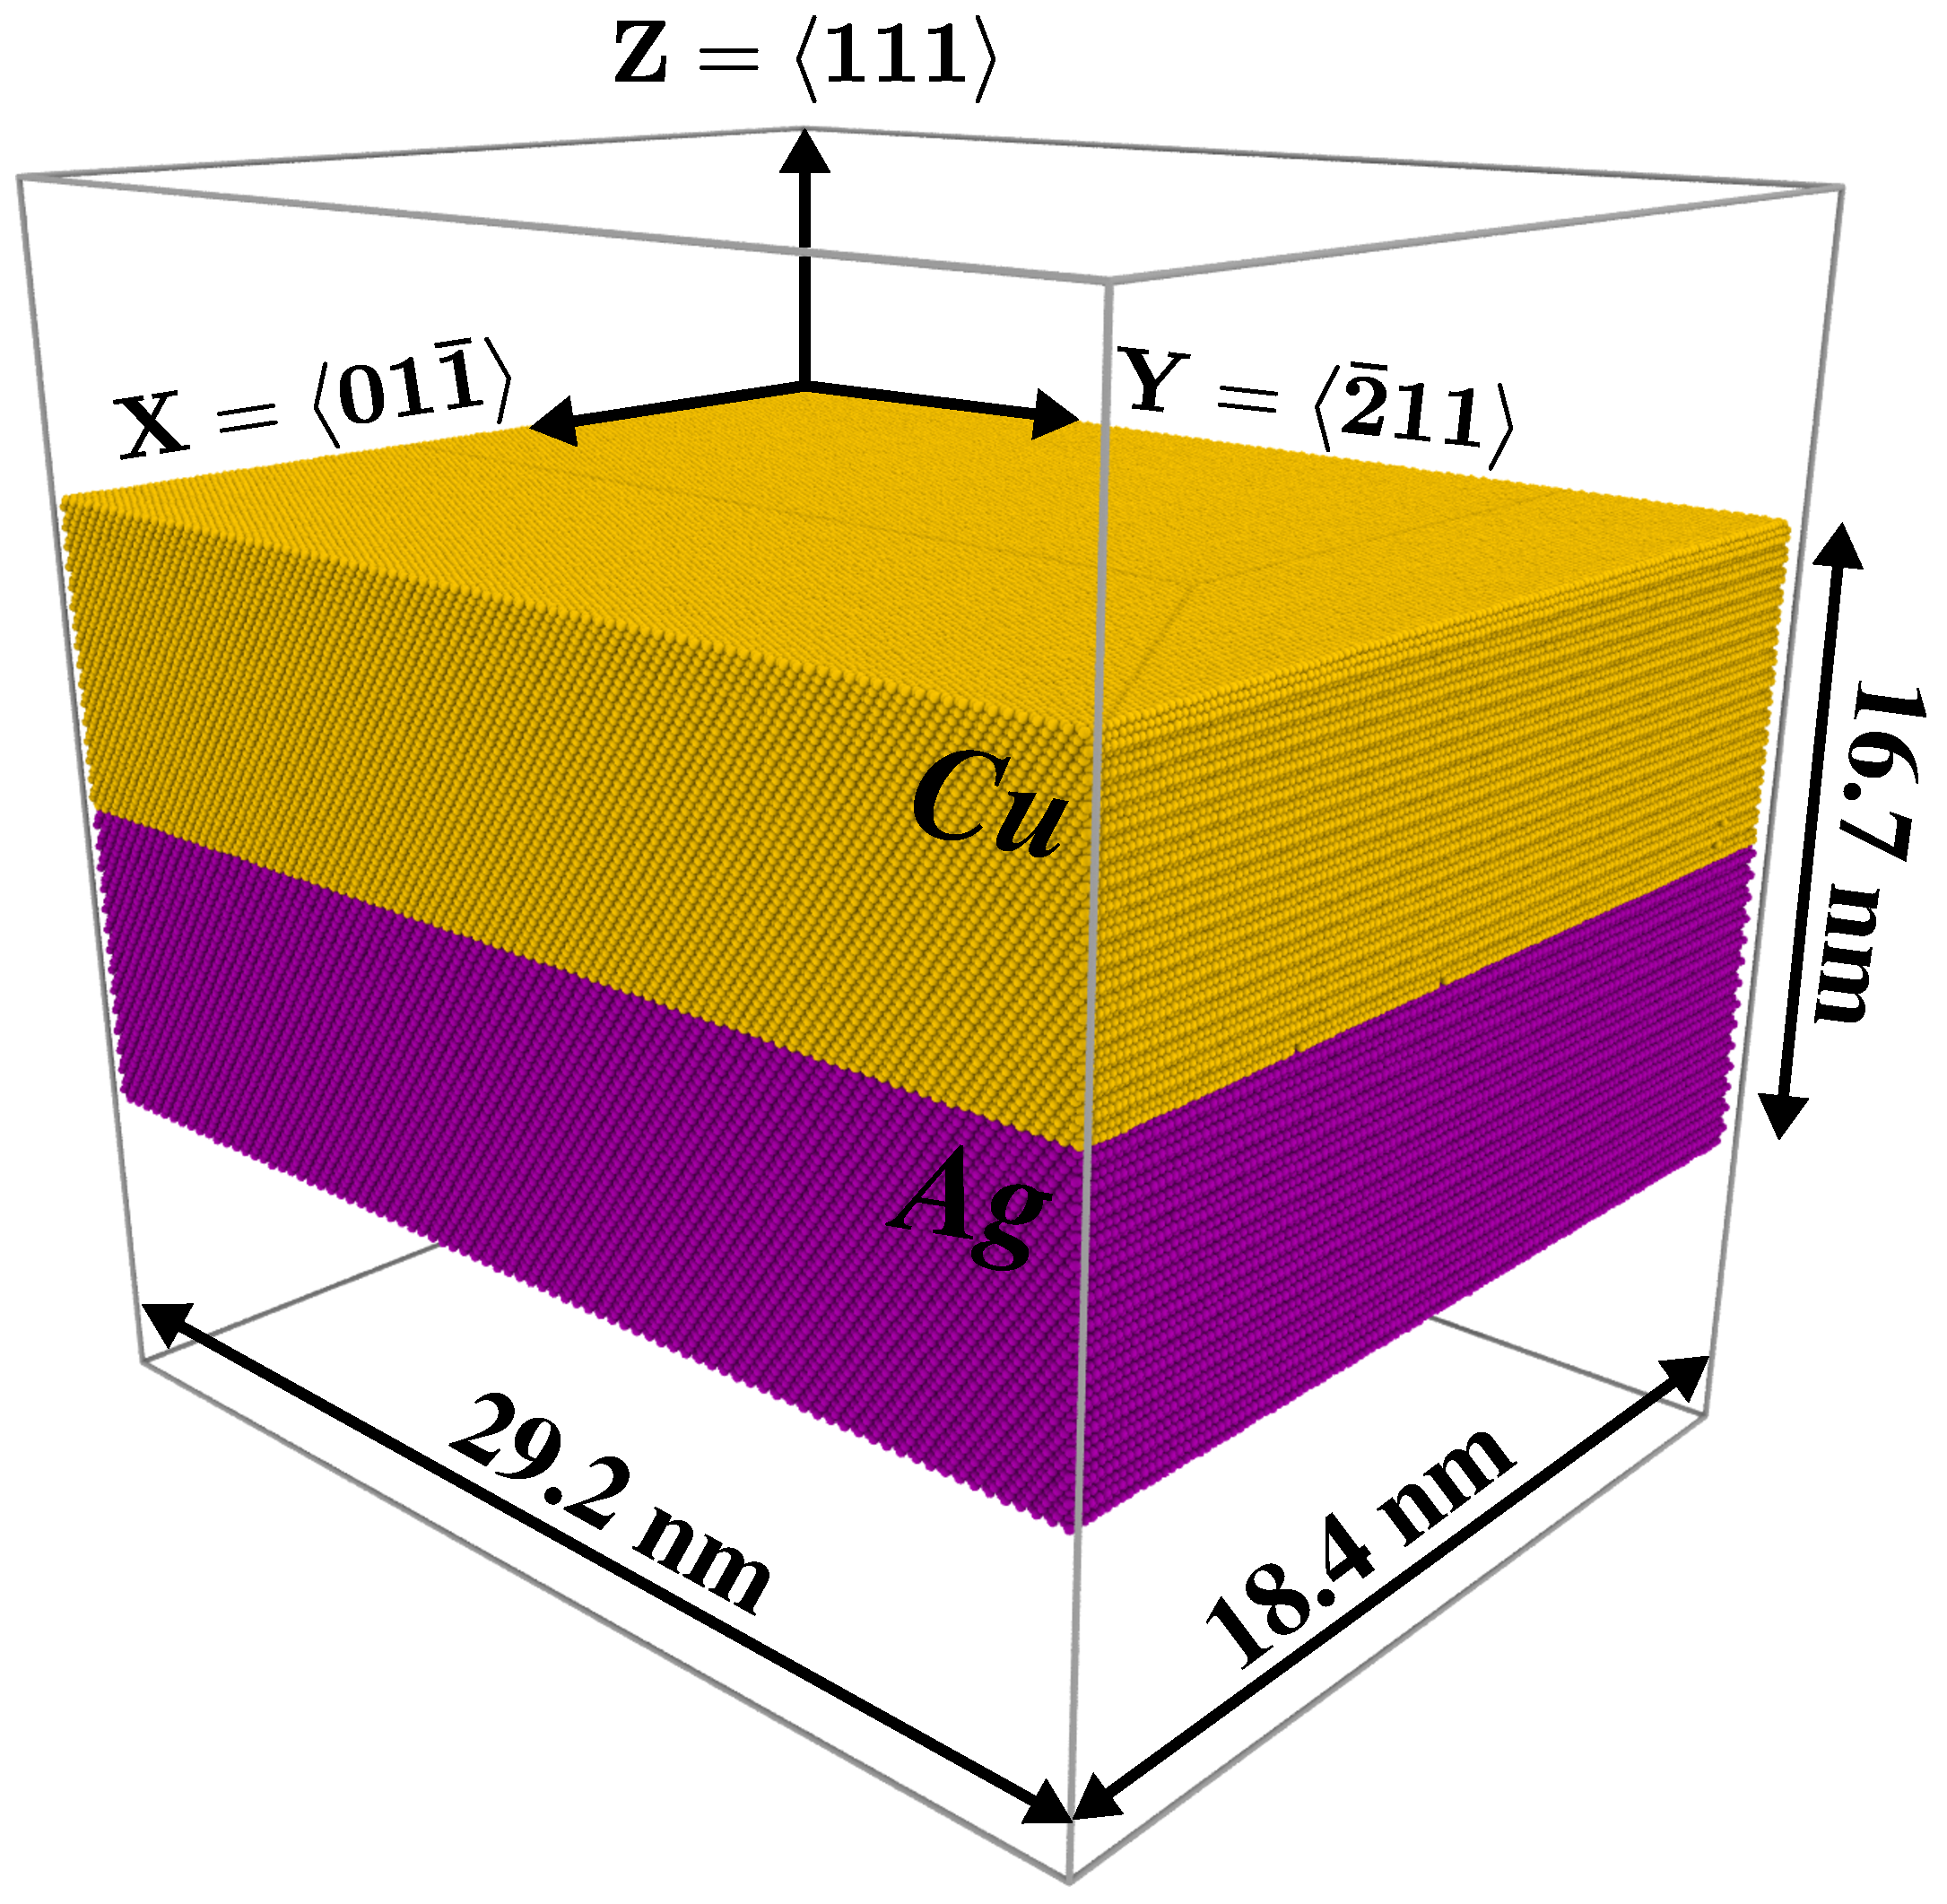
\includegraphics[width=70mm]{Pic/mod_geo.eps} 
	\end{center}
	\caption{Thin bimetallic film containing two layers with same dimensions along $X$, $Y$ and $Z$. Atoms are colored according to their types (Cu in purple and Ag in yellow).}\label{fig_mod_geo}
\end{figure}

Molecular dynamics calculations were then performed using the LAMMPS code \cite{plimpton95JCP}. The  embedded-atom method potential (EAM) of Williams et al. \cite{williams06MSMSE} was used to describe atomic interactions for Ag and Cu. For each of the two materials, this potential perfectly matches the lattice constants and closely reproduces the generalized stacking fault energies (GSFE) and the elastic constants, which are key parameters when one is interested in plasticity and more particularly on twin formation. More over in the case of bimetallic materials, this potential also permits to describe sliding, which is quantified by the GSFE and the Peierls stress \cite{li15PM}, at the $\lbrace111\rbrace$ Ag-Cu interface.

For each run, an energy minimization using a conjugate gradient algorithm was first performed to relax atomic positions at the interface. A 300 K temperature was then introduced by giving initial velocities to all atoms according to the Maxwell-Boltzmann distribution and the system was relaxed using an NPT integration according to the Nosé-Hoover thermostat, with zero pressure on each box faces. The system was subsequently compressed along the $Y=\langle\bar{2}11\rangle$ direction, by deforming the simulation box at $\dot{\varepsilon}=10^{8}~$s$^{-1}$ constant strain rate and using an NVT integration at 300 K, with a time step of 1 fs.

Different sets of atoms initial velocities for a given configuration were used to obtain a reliable statistics from our simulations. Similar plasticity mechanisms were thus observed, showing a good reproducibility. A larger system with a different aspect ratio (33.4 nm x 41.8 nm x 20.0 nm, for $\approx$ 1993990 atoms) was also tested and similar results were obtained. 

Post-processing was performed, using the Open Visualization Tool (OVITO) to visualize the atomic configurations \cite{stukowski10MSMSE1}. The Dislocation Extraction Algorithm (DXA) was used to identify bulk and interface dislocations with their associated Burgers vector and an ``home-made'' algorithm based on local rotations was developed to identify twins. Note however that this algorithm, described in annexe \ref{part_appendix}.

	\subsection{Interface description}
	\label{subpart_interface}

Ag and Cu have a significantly different lattice parameter, respectively $a_{Ag}=4.1~\AA$ and $a_{Cu}=3.6~\AA$, which implies a high misfit strain of 12.1\%. The stress generated by this lattice mismatch is relaxed by misfit dislocations at the interface. For Ag-Cu multi-layered materials only two semi coherent interfaces structures are possible: the cube on cube (COC) close-packed orientation and the twin orientation (TO). Both of them display a similar triangular mesh of misfit dislocations \cite{wang11SM,an15APL}.

\begin{figure}[!h]
	\begin{center}
		\includegraphics[width=70mm]{Pic/mod_inter.eps} 
	\end{center}
	\caption{Top view of Cu and Ag atoms along the interface in the case of a COC (a.i) and a TO (b.ii) interface. This view shows the Shockley partial dislocations mesh (highlighted by the black lines) and the stacking faults distribution at the interface. A side view along the $X=\langle01\bar{1}\rangle$ direction, shows coherent areas alternating with intrinsic stacking fault (ISF) areas in the case of a COC interface (b.i) and twin faults areas successively in the Cu part and in the Ag part in the case of a TO interface (b.ii). Atoms are coloured according to the centrosymmetry parameter.}\label{fig_mod_inter}
\end{figure}

To introduce the COC interface in our model, we construct two slabs, one for each material. Ag and Cu layers are therefore aligned along the $Z=[111]$ direction while the crystal orientations of both slabs are $X=[0\bar{1}1]$ and $Y=[\bar{2}11]$. The TO interface is built by keeping the previous orientation for the Ag layer while the Cu slab is rotated by 180° around the Y axis, leading to the following orientations: $X=[01\bar{1}]$, $Y=[\bar{2}11]$ and $Z=[\bar{1}\bar{1}\bar{1}]$. It can be noted that the Cu lattice is almost matching the Ag lattice since $8.a_{Ag}\simeq9.a_{Cu}$. 
%Looking to Ag and Cu lattice, the Cu lattice is almost matching the Ag lattice according to: $8.a_{Ag}\simeq9.a_{Cu}$. 
We can therefore adjust the global simulation box size by choosing initial lengths scaled to the average between $8.a_{Ag}$ and $9.a_{Cu}$, that is multiple of 
%multiples of the averaged distances between $8.a_{Ag}$ and $9.a_{Cu}$, wich correspond to: 
$\frac{\sqrt{2}}{2}\frac{(8.a_{Ag}+9.a_{Cu})}{2}$ in the $X=\langle0\bar{1}1\rangle$ and $\frac{\sqrt{6}}{6}\frac{(8.a_{Ag}+9.a_{Cu})}{2}$ in the $Y=\langle\bar{2}11\rangle$ \cite{li15PM}. 

Doing so, misfit dislocations are then directly introduced at the interface but without any core structure relaxation. The interface is therefore relaxed by performing an energy minimization using the conjugate gradient method while keeping zero pressure on each box faces. Fig. \ref{fig_mod_inter}.a shows the triangular mesh of intersecting dislocations obtained, for both interface types. The three types of dislocations introduced are identified as Shockley partial dislocations, with Burgers vectors $\overrightarrow{C\delta}$, $\overrightarrow{A\delta}$ and $\overrightarrow{\delta B}$ (according to the Thomson tetrahedron notation  \cite{hirth82book}) contained in the interface plane. These partial dislocations induce planar stacking faults at the interface. Depending on the interface type (COC or TO) the stacking faults are not similar and are differently distributed, as displayed in the side view of fig. \ref{fig_mod_inter}.b. The COC interface is composed of purely coherent areas alternating with intrinsic stacking fault (ISF) areas (Fig. \ref{fig_mod_inter}.b.i.), whereas the TO interface is entirely composed of twin faults with the faulted areas successively in the Cu part and in the Ag part (Fig. \ref{fig_mod_inter}.b.ii.).

\section{Influence of the interface type on mechanical twinning}
\label{part_influence}

Bimetallic systems with each type of interface were submitted to uni-axial compression along the $Y$ axis, as described in section~\ref{subpart_model}. The tests detailed in section~\ref{subsubpart_sAg} and \ref{subsubpart_sAg2} were realized with two mono-atomic steps on the Ag surface, separated by 14.7 nm. 
Typical deformation sequences are displayed in Fig.~\ref{fig_s1AgCOC}, with corresponding curves in Fig.~\ref{graph_stssnat}. Note however that because of thermal agitation, some variance in the systems behaviours can be observed.
In section~\ref{subsubpart_comparaison}, different nucleation sites were considered.

 
	\subsection{Cube on cube interface}\label{subsubpart_sAg}
    
\begin{figure*}[!t]
	\begin{center}
		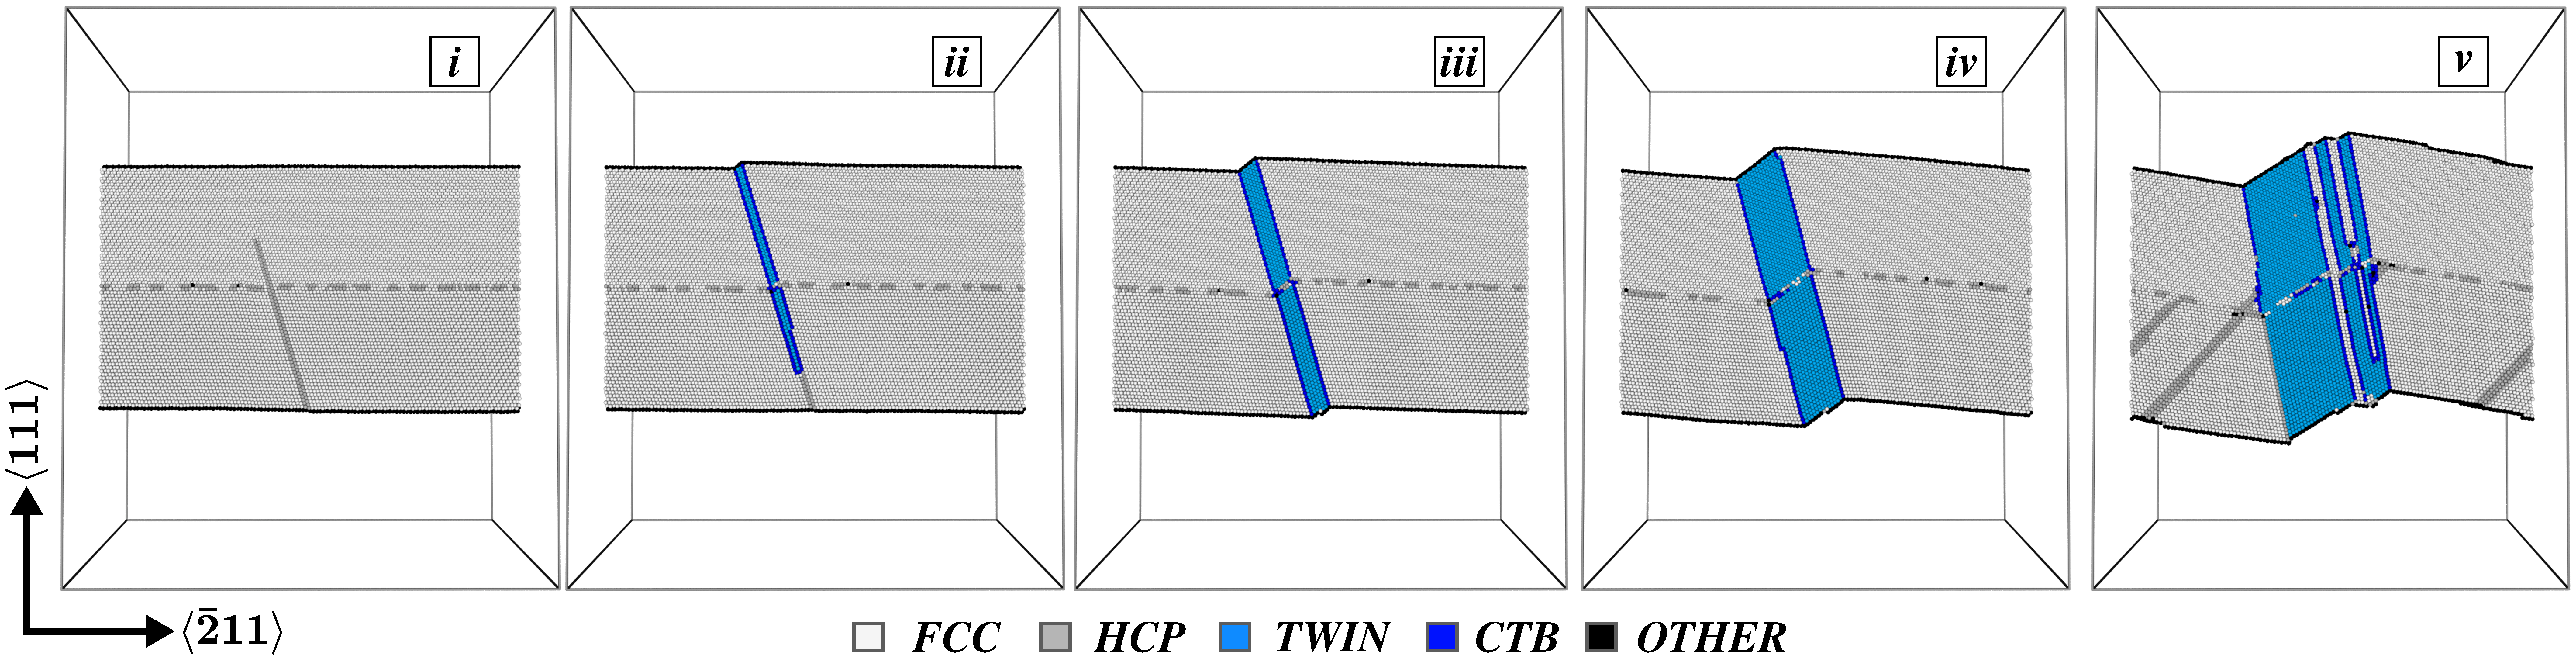
\includegraphics[width=150mm]{Pic/fig_s1AgCOC.eps} 
	\end{center}
	\caption{Plastic response of a thin Cu/Ag bimetallic film containing a COC (a) or a TO (b) interface, under a compression loading. 
(a.i-iii) Twin nucleation from a step on the Ag surface and twin thickening mechanism from the interface (a.iv). Subsequent plastic mechanisms with twin and perfect dislocations nucleation (a.v). (b.i-iii) Twin nucleation from a step on the Ag surface and Lomer dislocation nucleation from the interface (b.iii). Twin nucleation from the interface in the Cu layer (b.iii-v) and subsequent plastic mechanisms (b.v).
Atoms are coloured according to the common neighbour analysis (CNA) parameter. Atoms belonging to the surface or a dislocation line are coloured in black, atoms in ISF are in grey colour, and atoms in a perfect FCC structure are in light grey colour. Finally, atoms belonging to a twin correspond to light blue atoms and in navy blue to atoms in a CTB.}\label{fig_s1AgCOC}
\end{figure*}
For the system containing a COC interface, the onset of plasticity occurs for an average strain of 3.2\%. This average, as well as all those given throughout section~\ref{part_influence}, is calculated  over all simulations performed in the same configuration with different initial sets of velocities. As expected, the first plasticity event is the nucleation of a Shockley partial dislocation from one surface step. 
% On peut éventuellement préciser que la marche activée est bien celle prévue \cite{brochard00PMA,hirel07SM}.
This dislocation then glides, leaving behind an intrinsic stacking fault (ISF), through the whole Ag layer and crosses the interface (see Fig.~\ref{fig_s1AgCOC}.a.i). When this first dislocation reaches the Cu surface, two new Shockley partial dislocations are nucleated on both sides of the ISF, thus forming a small twin (see Fig. \ref{fig_s1AgCOC}.a.ii). This ``rebound'' or ``reflexion'' mechanism for twinning was first pointed out by Christian who extended the mechanism described by Frank for perfect dislocations gliding on a same $\lbrace111\rbrace$ plane \cite{hirth82book} to Shockley partial dislocations in adjacent planes \cite{christian51PRS}. Then twin extends via the nucleation from both surfaces of several Shockley dislocations in adjacent $\lbrace111\rbrace$  planes along the twin boundaries, always according to a ``rebound" mechanism. These onsets of plasticity and twinning correspond to the first stress drop in the light-blue stress-strain curve in Fig.~\ref{graph_stssnat}.a. When the stress becomes too low, twinning stops spontaneously for an average applied strain of 3.6\%; the corresponding snapshot is shown in Fig. \ref{fig_s1AgCOC}.a.iii. In figure \ref{graph_stssnat}.b, the light-blue curve reports the proportion of atoms belonging to a twin, obtained with our home-made algorithm, versus applied strain. A first increase can be seen between 3.3\% and 3.6\% strain, consistent with the mechanisms observed in Fig.~\ref{fig_s1AgCOC}.a.i-iii. 

\begin{figure*}[!t]
	\begin{center}
		\includegraphics[width=100mm]{Pic/fig_s1AgTO.eps} 
	\end{center}\caption{Misfit dislocations interacting with a Shockley partial dislocation (a) to give rise to the nucleation of a Lomer dislocation in the Ag layer and Shockley partial dislocation in the Cu layer (b). First Lomer dissociation mechanism leading to the nucleation of Shockley partial dislocation in the Ag part (c). Twin formation in the Cu and Ag part with the nucleation of Shockley partial dislocation in $\lbrace111\rbrace$ adjacent planes (d). As in Fig.\ref{fig_s1AgCOC}, atoms are coloured according to the CNA parameter and to our twin identification algorithm.}\label{fig_react_TO}
\end{figure*}


The stress in the whole system increases anew until twinning starts again at 5.1\% strain, with the nucleation of twin partial dislocations from surfaces. Another stress drop can therefore be observed in the stress-strain curve (Fig.~\ref{graph_stssnat}.a), and the proportion of ``twinned'' atoms increases a lot (Fig.~\ref{graph_stssnat}.b). This ends at an applied strain of 5.4\%, for which the stress starts rising up again, though more slightly than before the stress drops. In the same time, the proportion of ``twinned'' atoms increases slightly. This is explained by the activation of a different twinning mechanism, for which surfaces are not involved and Shockley partial dislocations are nucleated from the interface (Fig.~\ref{fig_s1AgCOC}.a.iv). This mechanism is described in detail in section~\ref{subsubpart_twin}. As evidenced in Fig.~\ref{graph_stssnat}, it is ``slower'' than the ``rebound'' mechanism and it is not sufficient to completely relax the stress induced by the applied strain.

For the specific test shown in Fig.~\ref{fig_s1AgCOC}, the ``interface'' twinning mechanism is observed after two sequences of ``surface'' twinning mechanism, with two stress drops in the stress-strain curves. This global twinning sequence will be later noted SSI (for Surface Surface Interface). It is worth noting that it is not always the case since for about half runs the ``interface'' twinning mechanism is observed after only one ``surface'' twinning mechanism sequence; this is evidenced by only one stress drop in the stress-strain curve, and no plateau in the ``twinned'' atoms proportion curve, as seen for example for some light-blue curves in Fig.~\ref{graph_limit_tsize}.a. This twinning sequence is noted SI.

Finally at higher applied strain (above 7.0\%), the stress is relaxed through the activation of other slip systems, with both Shockley partial and perfect dislocations (Fig.~\ref{fig_s1AgCOC}.a.v). These plasticity events are  accompanied by a stress drop and a significant increase of the proportion of ``twinned'' atoms (Fig.~\ref{graph_stssnat}).

	\subsection{Twin orientation interface}\label{subsubpart_sAg2}
	
The simulation was then performed for a thin film containing the TO interface. The onset of plasticity is similar to that observed with a COC interface: nucleation of a Shockley partial dislocation from one surface step for a same average strain of 3.2\% (see small stress drop in the red curve in Fig.\ref{graph_stssnat}.a). This is easily explained by the fact that the nucleation mechanism is very localized at the surface so that the interface plays no role in it. The dislocation then glides through the Ag crystal leaving behind an ISF, but unlike for the COC interface it is stopped and stored at the interface (Fig.~\ref{fig_s1AgCOC}.b.i). However, in the absence of any other plasticity mechanism, the stress in the whole system increases again.

\begin{figure*}[!t]
	\begin{center}
		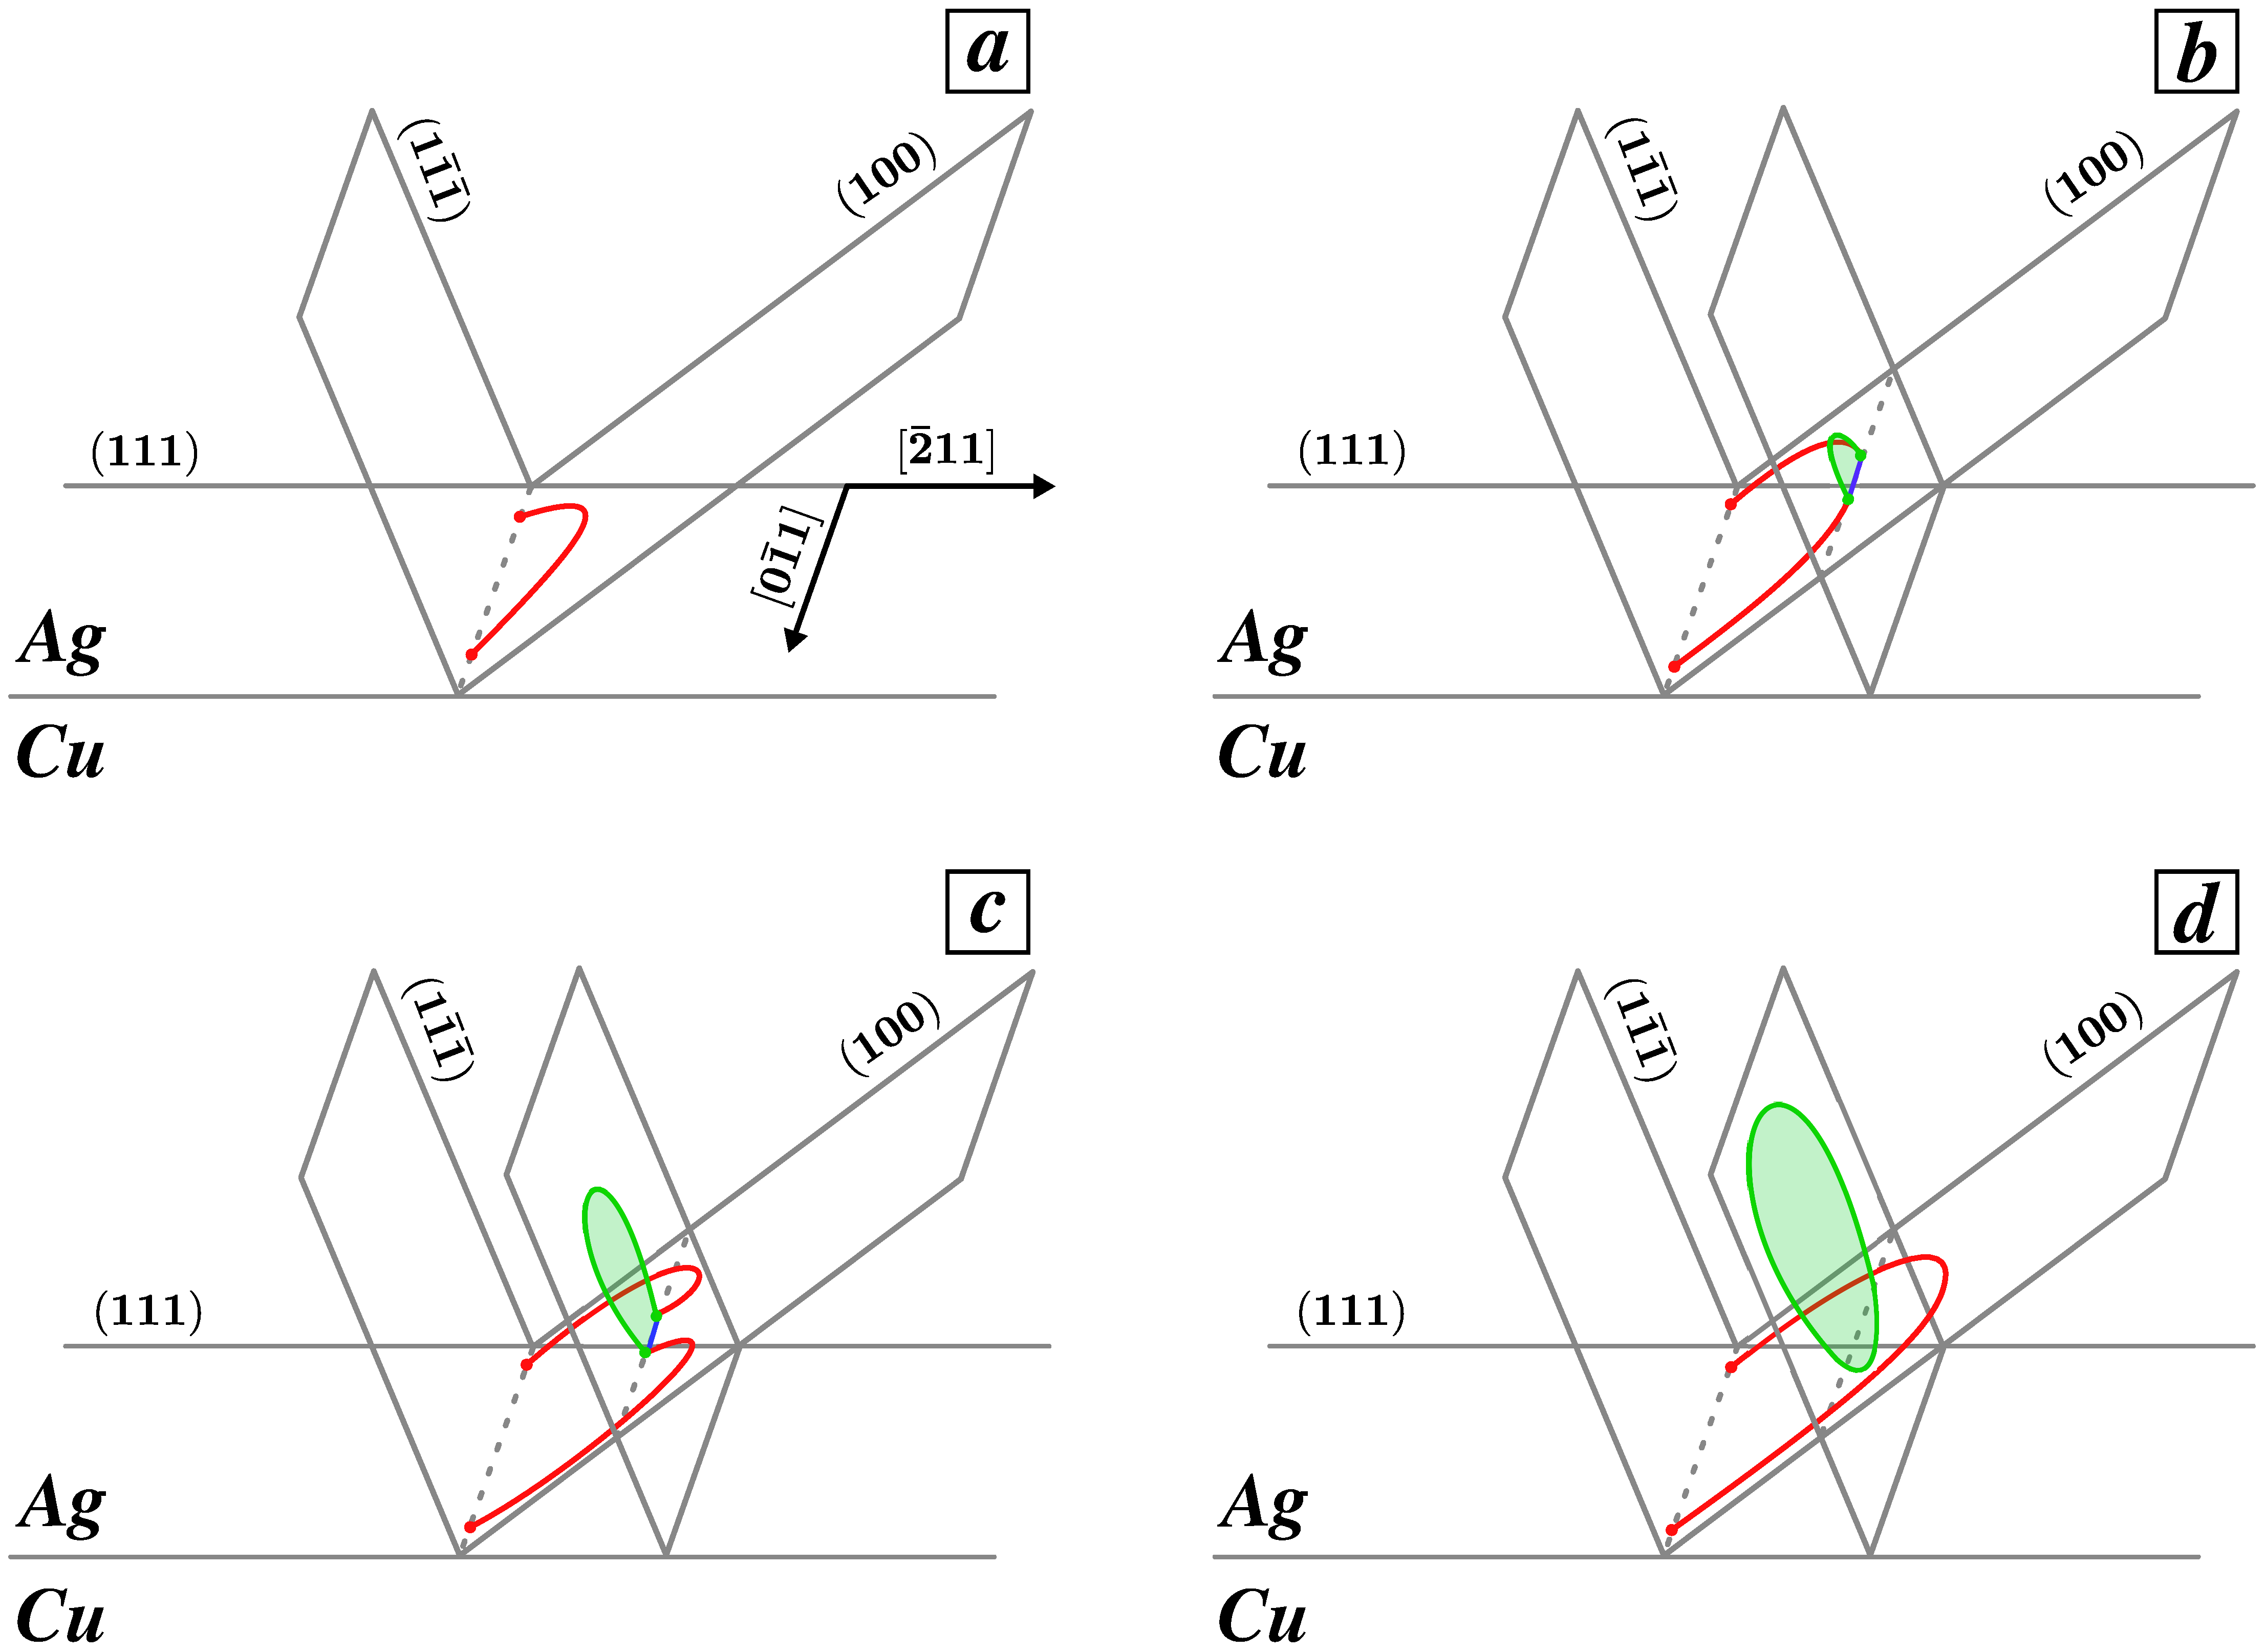
\includegraphics[width=150mm]{Pic/fig_lomdisso.eps} 
	\end{center}
	\caption{Schematic view of the Lomer partial dissociation mechanism leading to the formation of an isolated Shockley partial dislocation loop. (a) Starting configuration of Lomer dislocation (red line) gliding on a $(100)$ plane. (b) First Lomer dissociation mechanism leading to the nucleation of a Shockley partial dislocation in a $(1\bar{1}\bar{1})$ plane (light green line) leaving behind an ISF (transparent green area) and a sessile Frank partial dislocation (blue line). (c) Extension of the Shockley partial dislocation and the Lomer dislocation, the later being pined by the sessile Frank partial dislocation. (d) Removal of the sessile Frank partial dislocation leading to the formation of a isolated Shockley partial dislocation loop.}\label{fig_Lomer}
\end{figure*}
\begin{figure*}[!b]
	\begin{center}
		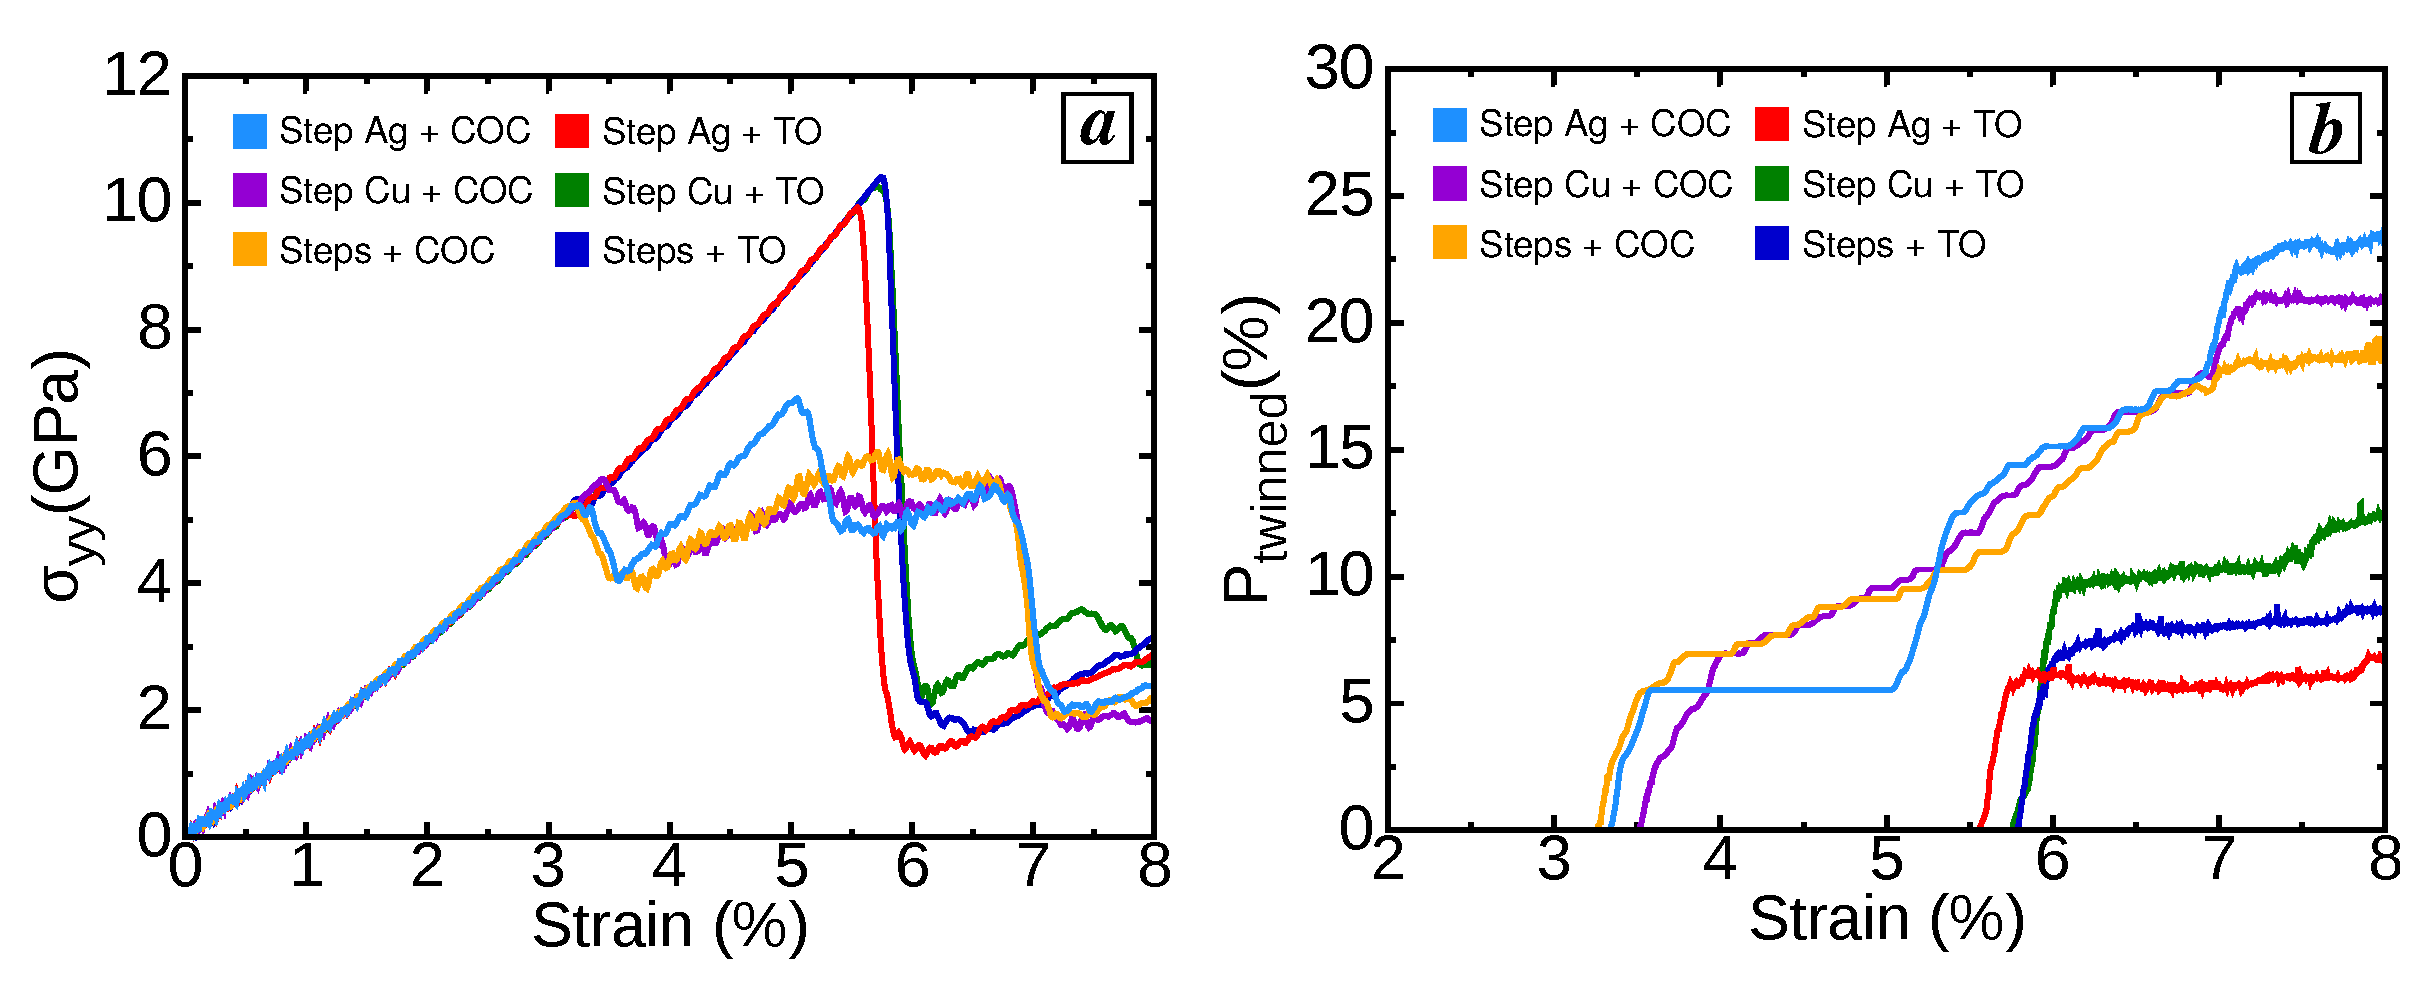
\includegraphics[width=150mm]{Pic/graph_natstss.eps} 
	\end{center}
	\caption{Stress (a) and total proportion of atoms belonging to a twin (b) as a function of strain. Light blue, purple and yellow curves correspond to film configurations containing a COC interface and with respectively surface steps on the Ag, Cu and both surfaces. Finally, red, green and navy blue curves correspond to film configurations containing a TO interface and with respectively surface steps on the Ag, Cu and both surfaces.}\label{graph_stssnat}
\end{figure*}

Plasticity starts again for an average strain of 5.5\%, as shown in Fig.~\ref{fig_s1AgCOC}.b.ii with the nucleation from the Ag surface of a Shockley partial dislocation forming a twin with the first nucleated dislocation. Right after (or for some tests right before), a Lomer dislocation in the Ag layer and a Shockley dislocation in the Cu layer are nucleated simultaneously from the interface (Fig. \ref{fig_s1AgCOC}.b.iii). The mechanism through which the first Shockley partial dislocation interacts with the interface leading to the formation of a Lomer dislocation in Ag and a Shockley dislocation in Cu is explained in detail in section~\ref{subsubpart_lomer}. 
Note that the Schmid factor is very high (0.47) for the Lomer dislocation, which promotes its gliding in the (100) plane.
As the Lomer dislocation crosses the entire Ag crystal from the interface to the surface, it causes the nucleation of several Shockley partial dislocations through successive occurrences of the mechanism illustrated in Fig~\ref{fig_Lomer}. Indeed, when gliding the Lomer dislocation partially dissociates into a Frank and a Shockley dislocation (Fig.~\ref{fig_Lomer}.b), according to \cite{wu09AM}:
\begin{eqnarray}\label{1}
	\begin{array}{ccccc}
\frac{1}{2}\left[0\bar{1}\bar{1}\right] &\rightarrow &  \frac{1}{3}\left[1\bar{1}\bar{1}\right]&+& \frac{1}{6}\left[\bar{2}\bar{1}\bar{1}\right] \\
BD &\rightarrow &  B\beta &+& \beta D\\
	\end{array}
\end{eqnarray} 
using Thompson tetrahedron notation. Along the portion of the Lomer dislocation line aligned along the $\left[01\bar{1}\right]$ direction,the purely edge Shockley partial dislocation resulting from the dissociation can glide in the $\left(bar{1}11\right)$ plane leaving behind a sessile Frank dislocation. The Shockley partial can glide easily in the Ag crystal part whereas the Frank partial dislocation is purely sessile. So both the Lomer dislocation portion which has not been dissociated yet and the Shockley dislocation are pinned by the Frank partial while they are still gliding (Fig.~\ref{fig_Lomer}.c). The Shockley, Frank and Lomer dislocations are pinned at triple nodes that can only move along the $\left[01\bar{1}\right]$ direction. As the Shockley and Lomer dislocations bow out in their respective planes the distance between the two triple nodes decreases and the Frank segment finally disappears according to the reaction reverse to reaction~\ref{1}. The Shockley partial forms a loop, which can extend in the whole crystal, and parts of the Lomer dislocation recombine in a fashion similar to that of Frank-Read sources \citep{frank50} (Fig.~\ref{fig_Lomer}.d). While it is still gliding in its (100) plane, the Lomer dislocation can thus continue to generate Shockley partials in parallel $\lbrace111\rbrace$ planes and can eventually led to the formation of twins if these planes are adjacent. We observe that this mechanism operates few times while the Lomer dislocation crosses the Ag layer, inducing the nucleation of several Shockley dislocations (Fig.~\ref{fig_s1AgCOC}.b.iv) and in some cases twins. Simultaneously, few Shockley dislocations are nucleated from the surface and along the first ISF in the Ag crystal, thus forming a twin (Fig.~\ref{fig_s1AgCOC}.b.v). In the Cu part, the Shockley dislocation reaches the surface and induces the nucleation of new Shockley dislocations in $\lbrace111\rbrace$ adjacent planes, thereby forming a twin (Fig.~\ref{fig_s1AgCOC}.b.iii-v). All the formed twins are finally stopped at the interface.

These plasticity mechanisms all operate at the same time at 5.5\% applied strain, resulting in an important stress drop which can be seen in the stress-strain curves (red curve in Fig. \ref{graph_stssnat}.a). There is also a significant increase of the ``twinned'' atom proportion because of the concomitant nucleation of twins in the Cu and Ag layers (red curve in Fig. \ref{graph_stssnat}.b), although the proportion of ``twinned'' atom is much less than for a COC interface at the same applied strain.
 
 
	\subsection{Varying nucleation sites}\label{subsubpart_comparaison}
	
In order to test the influence of the first plasticity event location, steps were introduced on the Cu surface, along with or without steps on the Ag surface.
	
For all tested cases, Shockley dislocations are nucleated from   steps. When steps are introduced on the Cu surface only, the yield point is slightly higher ($\sim 3.3\%$) than when steps are present on the Ag surface. This is consistent with higher intrinsic and unstable stacking fault energies in Cu [Ref ?]. When steps are introduced on both surfaces, the first plasticity event therefore always starts at one of the Ag surface step, and the yield point is similar to that described in part \ref{subsubpart_sAg} and \ref{subsubpart_sAg2}(yellow and navy-blue curves in Fig.~\ref{graph_stssnat}.a). 

For systems with a COC interface, the plastic response to the applied strain is similar whatever the first dislocation nucleation site. The two distinct twinning mechanisms (surface ``rebound'' and interface nucleation) are observed, but the twinning sequence can be different: SSI or SI (see part \ref{subsubpart_sAg}). 
%but the second one operates at different applied strain levels depending on the test. In particular, the activation of the ``interface'' twinning mechanism is delayed when two sequences of ``rebound'' mechanism occur before, as for the case described in section~\ref{subsubpart_sAg} (compare light-blue and yellow or purple curves in Fig.~\ref{graph_stssnat}). 
It is worth noting that if steps are present on the Cu surface only, the ``interface'' twinning mechanism is always activated after only one ``rebound'' mechanism sequence (see purple curves in Fig.~\ref{graph_stssnat}), according to a SI twinning sequence. As it will be discussed in part \ref{subsubpart_twin}, this is partly due to a higher yield strain. It should also be noted that when steps are introduced on both sides, the onset of plasticity in Ag is quickly followed by twin formation which relaxes a significant amount of stress (see yellow curve in Fig.~\ref{graph_stssnat}.a), so that the steps on the Cu surface are in general not activated.

For systems containing a TO interface, the onset of plasticity is not strongly influenced by the location of the first nucleated dislocation: Shockley partial dislocations are always first nucleated from surface steps, glide through half part of the system and are stopped and stored at the interface. If surface steps are present on both sides of the system, this occurs almost simultaneously in both Cu and Ag parts; two Shockley dislocations are thus nucleated.
As for the subsequent events, they depend significantly on the first nucleation sites: Lomer dislocations are formed only in the Ag crystal, when a Shockley partial in the Ag part interacts with the interface. When steps are introduced on the Cu surface only, the first Shockley dislocation nucleates from the step in the Cu crystal. A new Shockley partial can later be nucleated from a random site on the Ag surface, for high enough accumulated stress. Then it glides and reaches the interface where its interaction with misfit dislocations gives rise to Lomer dislocation and another Shockley partial according to the mechanism described in section~\ref{subsubpart_sAg2}.
% With an equal probability, another possible mechanism is the nucleation of an extrinsic stacking fault (ESF) directly from the Ag surface with the successive nucleation of two Shockley dislocations in $\lbrace111\rbrace$ adjacent planes. They are next stopped at the interface and induce the nucleation of a Lomer dislocation in the Cu part of the film \textcolor{red}{(à vérifier, car contredit ce qu'on a mis plus haut)}; this mechanism will be described in detail in section~\ref{subsubpart_lomer}.
 
\section{Role of misfit dislocations}
\label{part_misfit}

It has been previously showed, in the presence of surface defects interfaces are not directly involved on the first dislocation nucleation mechanisms. However, interactions between particular defects (Shockley dislocation or CTB) with interfaces and more particularly misfit dislocations can lead to particular plasticity mechanisms. A full description of the Lomer dislocation nucleation mechanism, which was observed for the TO interface in part \ref{subsubpart_sAg2}, is made in part \ref{subsubpart_lomer}. In the same way, the twinning mechanism operating from the interface and contributing to the twin extension in the case of a COC interface (see part \ref{subsubpart_sAg}) is detailed in part \ref{subsubpart_twin}.  

	\subsection{Nucleation of Lomer dislocation - TO interface}
	\label{subsubpart_lomer}
	
In the case of a TO interface, dislocation transmission is not possible due to an high angle disorientation between the two layered crystals. Dislocations nucleated from the surface of the film are therefore stopped and stored at the interface where they can interact with misfit dislocations or between them to induce particular plasticity mechanisms. In our systems only Shockley partial dislocations are nucleated from the surface. These dislocations can therefore combine with misfit dislocations (see Fig. \ref{fig_react_TO}.a), according to the following reaction:

\begin{eqnarray}\label{2}
	\begin{array}{ccccccccccccc}
\frac{1}{6}\left[211\right]_{Ag} &+& \frac{1}{6}\left[2\bar{1}\bar{1}\right]_{Ag} &\rightarrow& \frac{2}{3}\left[100\right]_{Ag},\\
D\beta_{Ag} &+& B\delta_{Ag} &\rightarrow& \frac{2}{3}BD/AC_{Ag} 
	\end{array}
\end{eqnarray}

When the accumulated stress is high enough, this newly formed dislocation dissociates to induce the nucleation of a Lomer dislocation in the Ag part and a second Shockley partial dislocation in the Cu part (see Fig. \ref{fig_react_TO}.b):

\begin{eqnarray}\label{3}
	\begin{array}{ccccccccccccc}
\frac{2}{3}\left[100\right]_{Ag} &\rightarrow& \frac{1}{2}\left[0\bar{1}\bar{1}\right]_{Ag} &+& \frac{1}{6}\left[\bar{2}\bar{1}\bar{1}\right]_{Cu}  &+&\\
 & & \frac{1}{6}\left[2\bar{1}\bar{1}\right]_{Ag} &+& D_{res},\\
\frac{2}{3}BD/AC_{Ag} &\rightarrow& BD_{Ag} &+& \beta D_{Cu} \\
 & & B\delta_{Ag} &+& D_{res}
	\end{array}
\end{eqnarray} \\

The Shockley partial dislocation then crosses the entire Cu layer and causes the formation of a twin via the nucleation of successive Shockley dislocations from the free Cu surface (see Fig. \ref{fig_react_TO}.c). The interface thus plays directly the role of a source for twin nucleation. 

Another mechanism of dislocation recombination which can leads to the nucleation of Lomer dislocation has been observed in some configurations. This mechanism occur in the Cu layer when two Shockley partial dislocations are nucleated successively in $\lbrace111\rbrace$ adjacent planes, thus forming a ESF. These two Shockley partials dislocations collapse to form a super dislocation ($ 2~\beta D_{Cu} $) at the interface, according to the reaction:

\begin{eqnarray}\label{3}
	\begin{array}{ccccc}
\frac{1}{6}\left[211\right]_{Cu} &+& \frac{1}{6}\left[211\right]_{Cu} &\rightarrow& \frac{1}{3}\left[211\right]_{Cu}, \\
D\beta_{Cu} &+& D\beta_{Cu} &\rightarrow & 2~D\beta_{Cu} \\
	\end{array}
\end{eqnarray}

The super dislocation rapidly dissociates into a sessile stair-rod dislocation ($\beta\delta_{Cu}$) stored at the interface and a Lomer dislocation $ BD_{Ag} $ which can glides on a $\lbrace100\rbrace$ in the second part of the film, such as:

\begin{eqnarray}\label{2}
	\begin{array}{ccccc}
\frac{1}{3}\left[211\right]_{Cu} &\rightarrow & \frac{1}{6}\left[011\right]_{Cu} &+& \frac{1}{2}\left[0\bar{1}\bar{1}\right]_{Ag}, \\
2~D\beta_{I} &\rightarrow & \beta\delta_{Cu} &+& BD_{Ag} \\
	\end{array}
\end{eqnarray}

\textcolor{blue}{Je ne sais pas si ce dernier mécanisme est vraiment pertinent pour moi il est assez annecdotique, en effet il n'opère que dans certains cas et à forte déformation.}  

In this case, dislocation-interface interactions always lead to the nucleation of Lomer dislocations which largely contribute to the plastic deformation of the thin film. Lomer dislocations has already been observed experimentally \cite{bonneville90PML,mills89PMA}, and in few simulations in deformed fcc metals. It has been found that they generally result from the interaction of a perfect dislocation and a CTB \cite{sansoz07NL,wu09AM}. However, they are not stable and when it is possible they generally dissociate to form Lomer-Cottrell lock, in bulk materials \cite{hirth82book,wu09AM}. In our really small systems the dissociation mechanism is not or partially occurring \ref{subsubpart_sAg2}. This is partly due to an high accumulated stress. % associated with an high Schmid factor which is sufficient to induce easily their gliding along $\lbrace100\rbrace$ planes. 
Furthermore due to close surfaces, dislocations are rapidly eliminated which reduce their dissociation probability while gliding. As described in part \ref{subsubpart_sAg2}, these dislocations can also act as sources for Shockley dislocations according to the first dissociation mechanism (see eq. \ref{1} and Fig. \ref{fig_Lomer}) and possibly deformation twins. 

\begin{figure}[!h]
	\begin{center}
		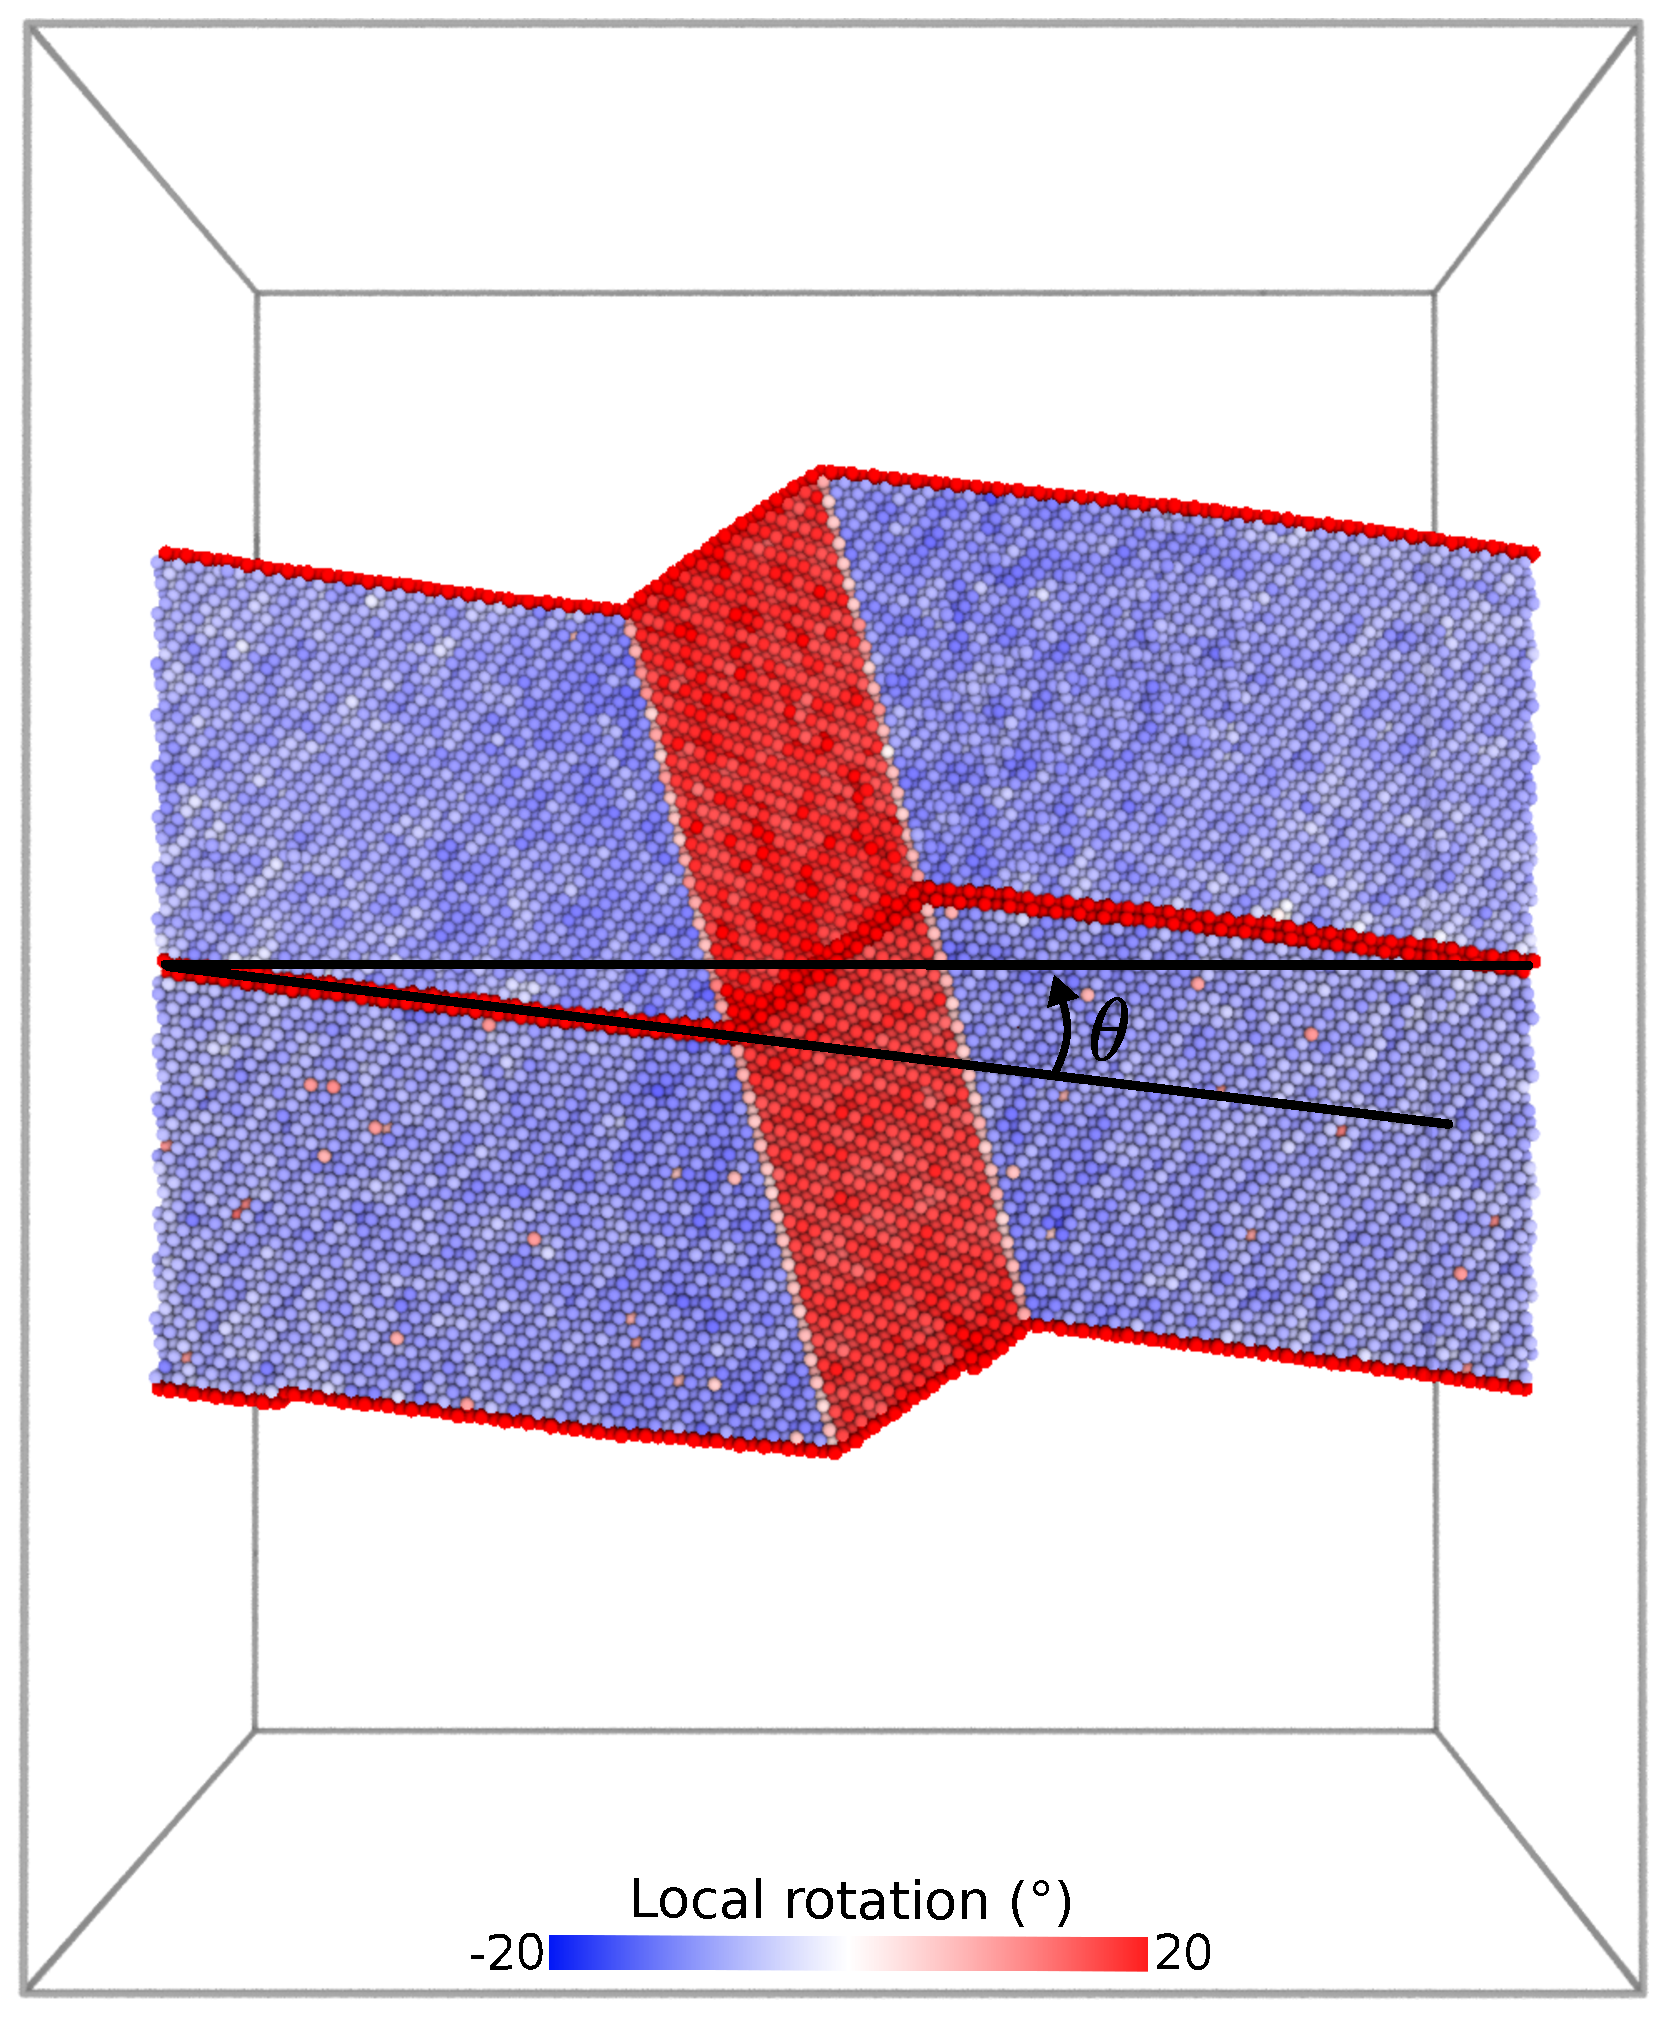
\includegraphics[width=70mm]{Pic/graph_res_rot_fig3.eps} 
	\end{center}\caption{Thin Cu/Ag film containing a COC interface deformed plastically by twinning and rotated around the $X=\langle0\bar{1}1\rangle$ axis with an angle $\theta$. Atoms are coloured according to the rotation of their local environment (compared to a non deformed initial configuration see part \ref{part_appendix}).}\label{graph_res_rot}
\end{figure}

\begin{figure}[!h]
	\begin{center}
		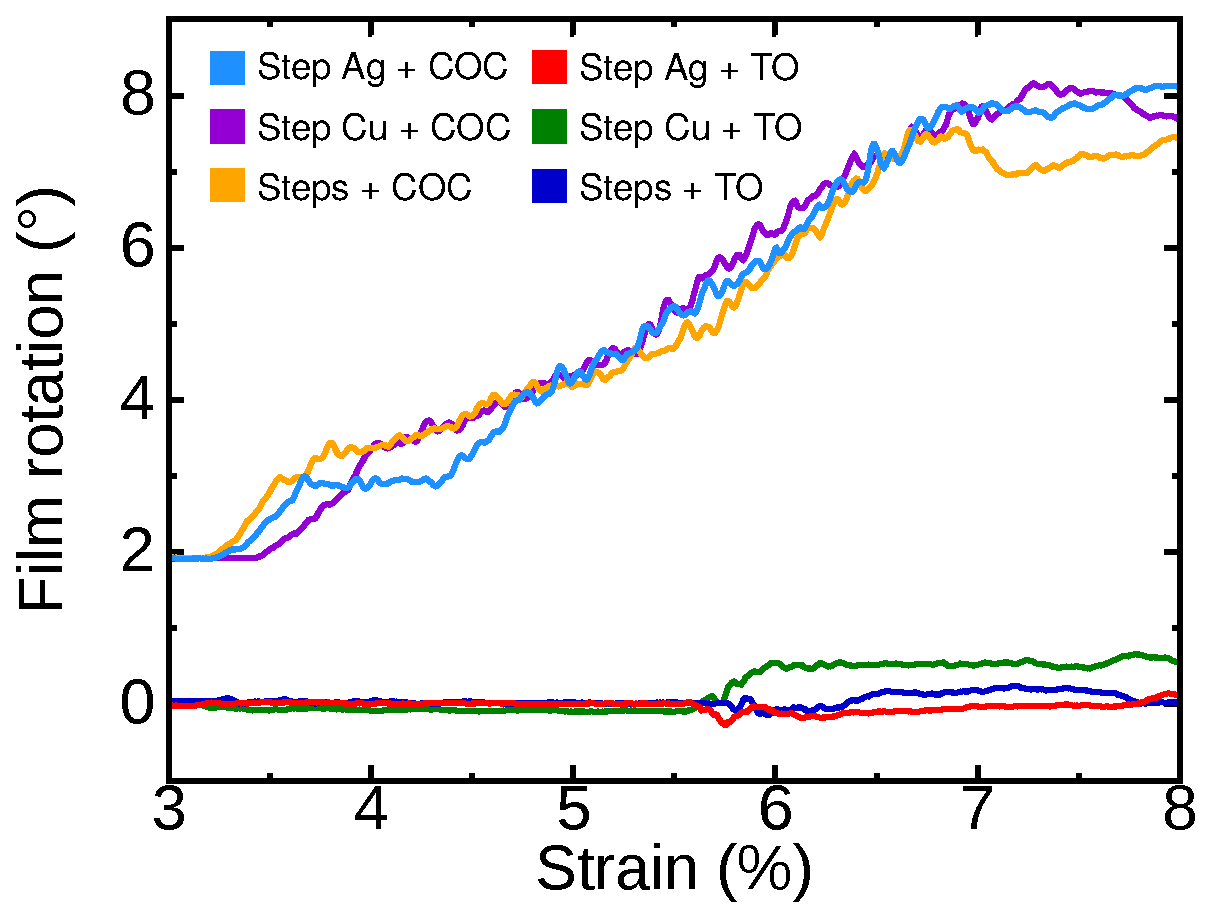
\includegraphics[width=70mm]{Pic/graph_rotation.eps} 
	\end{center}\caption{Global rotation evolution of the thin film against the strain for a thin Cu/Ag films containing a COC interface or a TO interface. The same color coding as in Fig.\ref{graph_stssnat} has been used for curves.}\label{graph_rotation}
\end{figure}

	\subsection{Twin dislocation nucleation induced by misfit dislocation - COC interface}\label{subsubpart_twin}
	
\begin{figure*}[!b]
	\begin{center}
		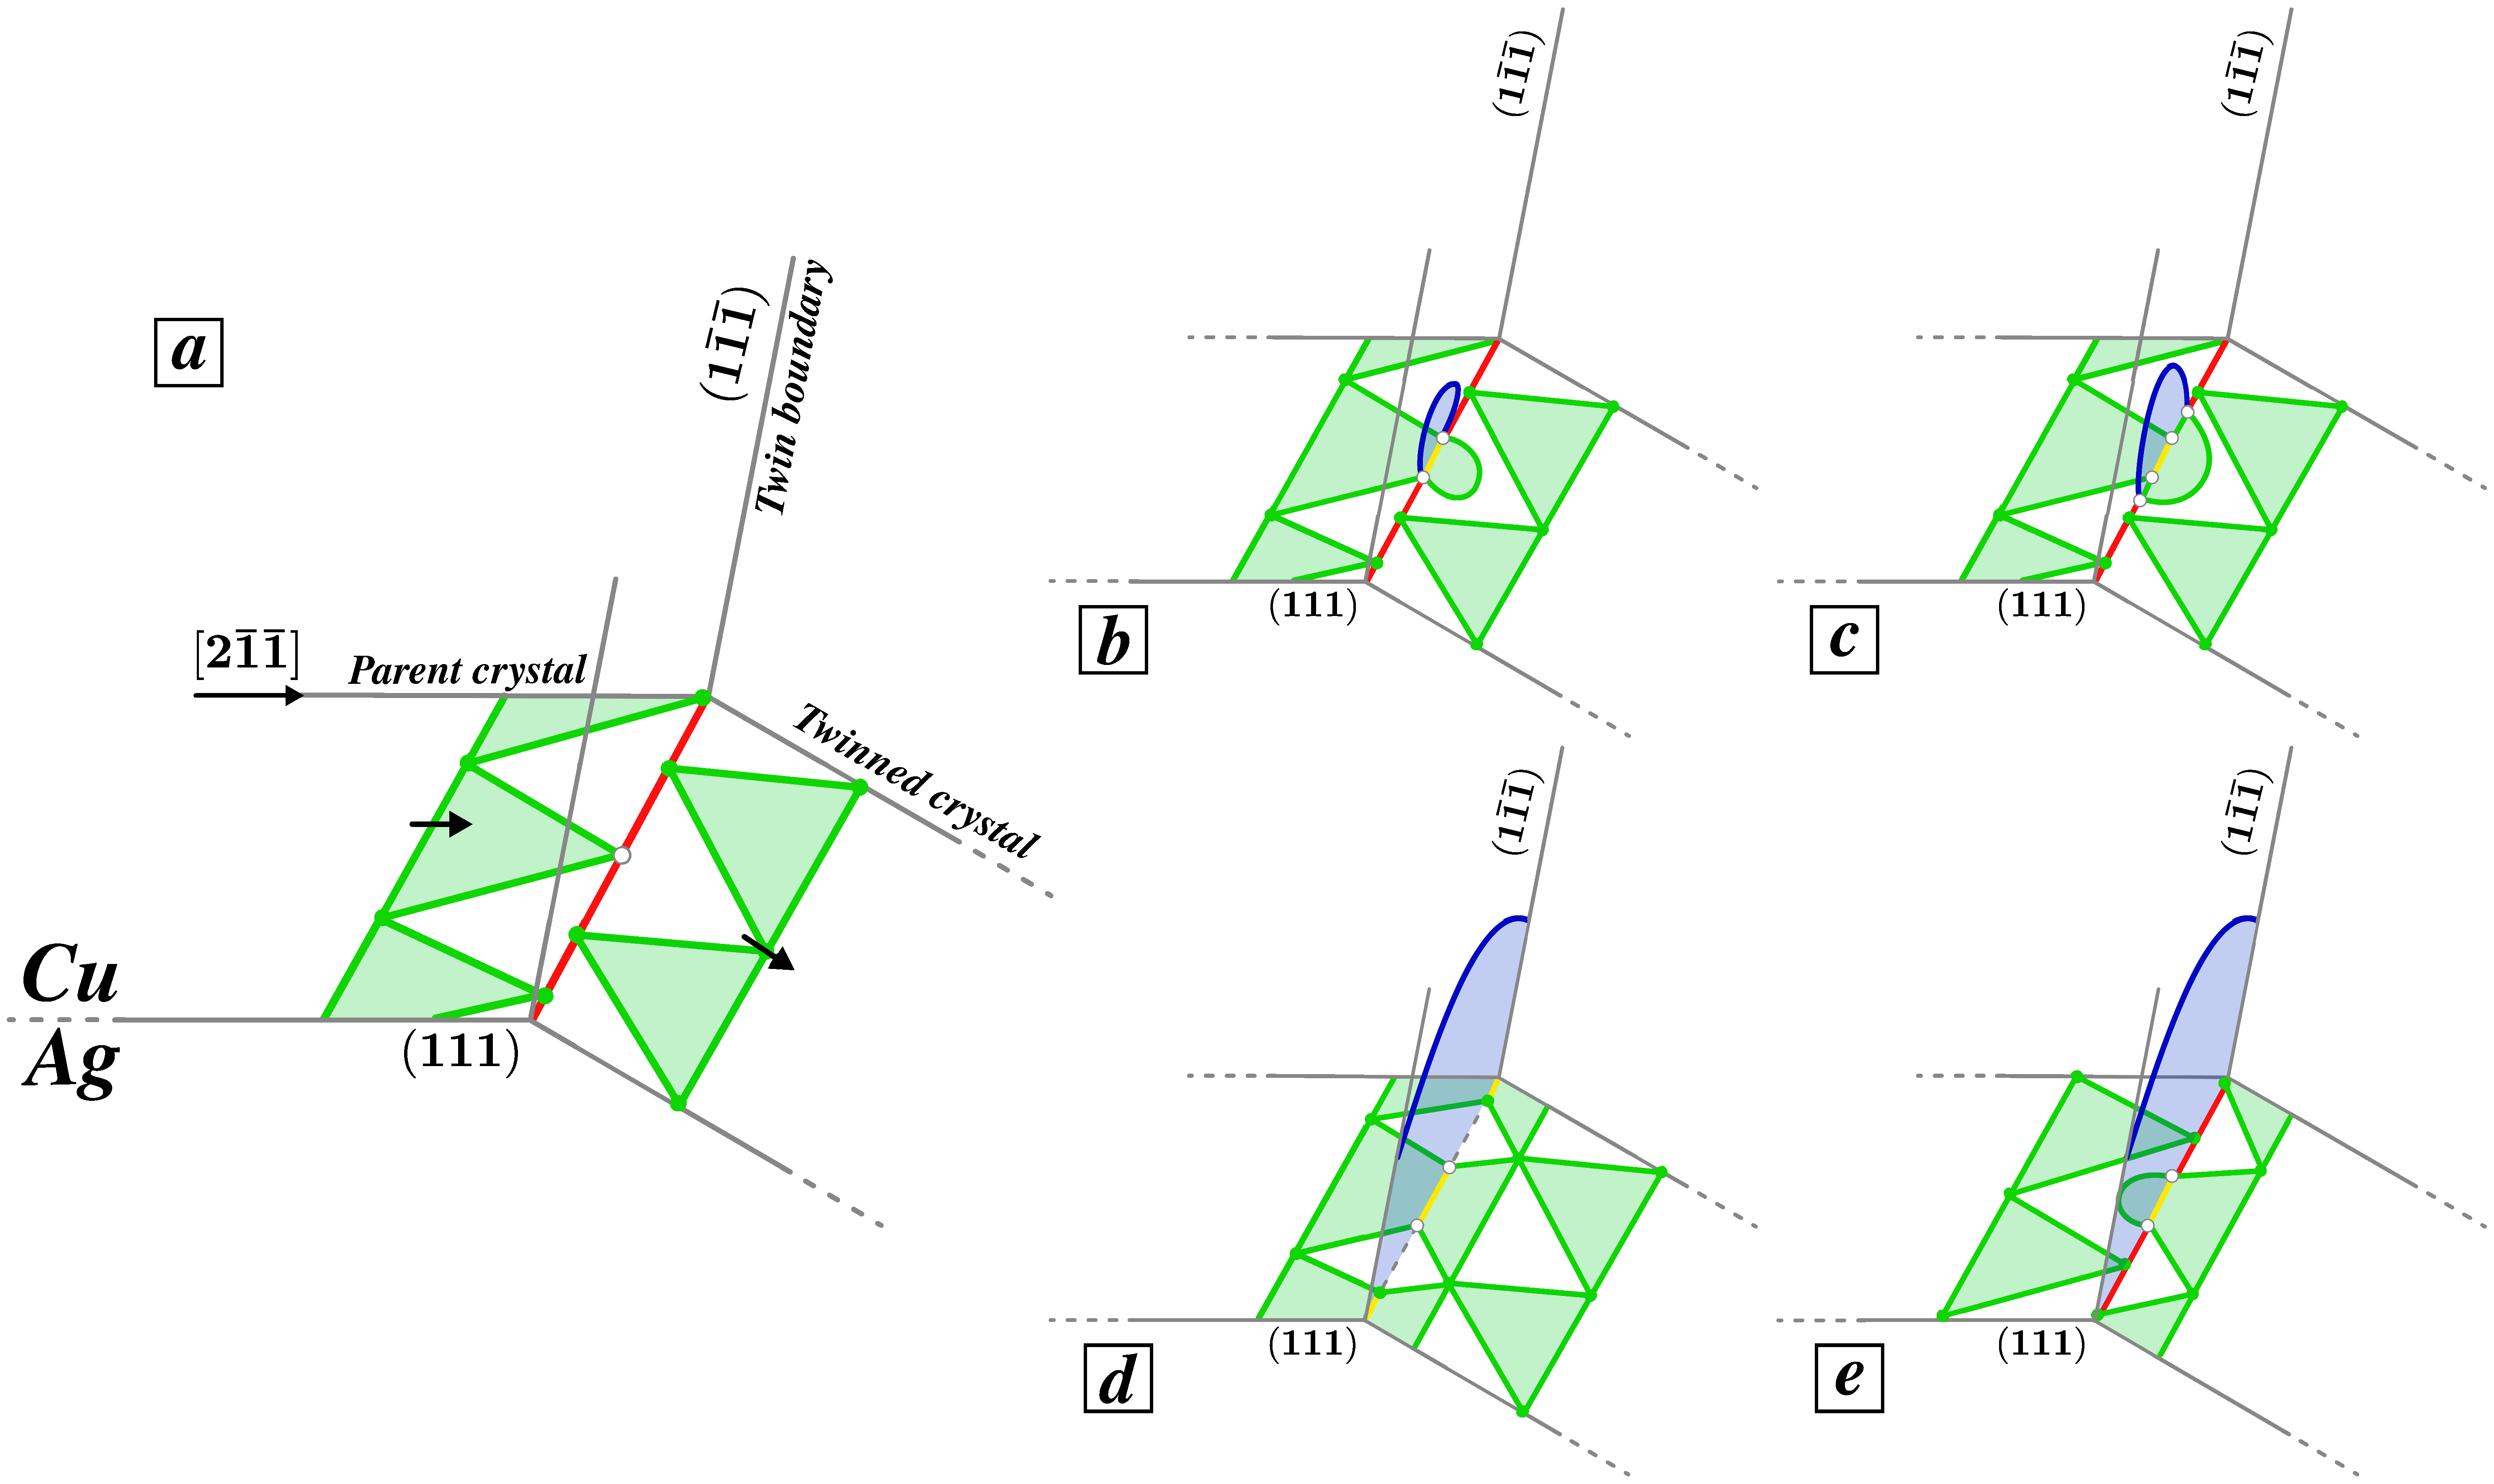
\includegraphics[width=150mm]{Pic/fig_ENT.eps} 
	\end{center}\caption{Schematic view of the interactions of misfit dislocations with a twin boundary, leading to the nucleation of twin dislocation in the Ag layer. A full description of these interactions mechanisms is made in part \ref{subsubpart_twin}. The light green lines correspond to Shockley partial dislocations gliding along the interface plane with their associated ISF (green areas), whereas the blue line corresponds to one gliding along the twin boundary plane and the blue area corresponds the ISF. The red line is associated to perfect lattice dislocation and the purple line to a residual dislocation blocked along the interface and the twin boundary plane.}\label{fig_ENT}
\end{figure*}

Unlike the TO interface, a COC interface is fully permeable to dislocations, interface-dislocations interactions are therefore very limited. However as seen in section \ref{subsubpart_sAg}, the interface can act as sources for twin dislocations.

%As we have just showed, the twinning mechanism from interfaces involves misfit dislocations. To take place, dislocations gliding needs to be stress activated which is only possible if the resolved shear stress in the interface plane is sufficient. However, given that the compression axis is along the interface plane according to the chosen orientations, the resolved shear stress on misfit dislocation should be close to zero. This point no longer becomes true as soon as plasticity occurs. 

In the the case of a COC interface, we showed that twinning is occurring from the surfaces and then from the interface (see part \ref{subsubpart_sAg}). Therefore due to the twin formation and the periodic boundary condition, a rotation of the whole film is observed. We have calculated this rotation by averaging over all the atoms not belonging to a twin a local rotation (see Fig. \ref{graph_res_rot}) which is extracted using an ``home-made" algorithm (see part \ref{part_appendix}). This rotation has been plotted as a function of the strain (see Fig. \ref{graph_res_rot}.b). In the presence of a COC interface, this graphic clearly shows a global rotation of the whole film around the $X=\langle01\bar{1}\rangle$ axis rotation which is first induced elastically by a pre-shearing of the $\lbrace111\rbrace$ planes and then plastically with the twin nucleation (see purple, light blue and yellow curves on Fig. \ref{graph_rotation}), after reaching the yield strain ($ \sim 3.2\% $). The resolved shear stress on the interface plane (which is initially close to $0~GPa$) then increases sufficiently to induce gliding of misfit dislocations. These one can therefore glide along the interface until being stopped at the newly formed twin boundary, where they can interact with the later to give rise to the nucleation of a twin partial dislocation. In a same way, the resolved shear along the interface in the twinned crystal portion is also not zero. In fact, this one undergoes the rotation induced by twinning less the rotation of the whole thin film ($\theta_{twin}=19.47^{\circ}-\theta$). This rotation is as well sufficient to induce gliding for misfit dislocations in the twinned crystal part, which can also interact with the second twin boundary and participate to the twin extension. 

\begin{figure*}[!t]
	\begin{center}
		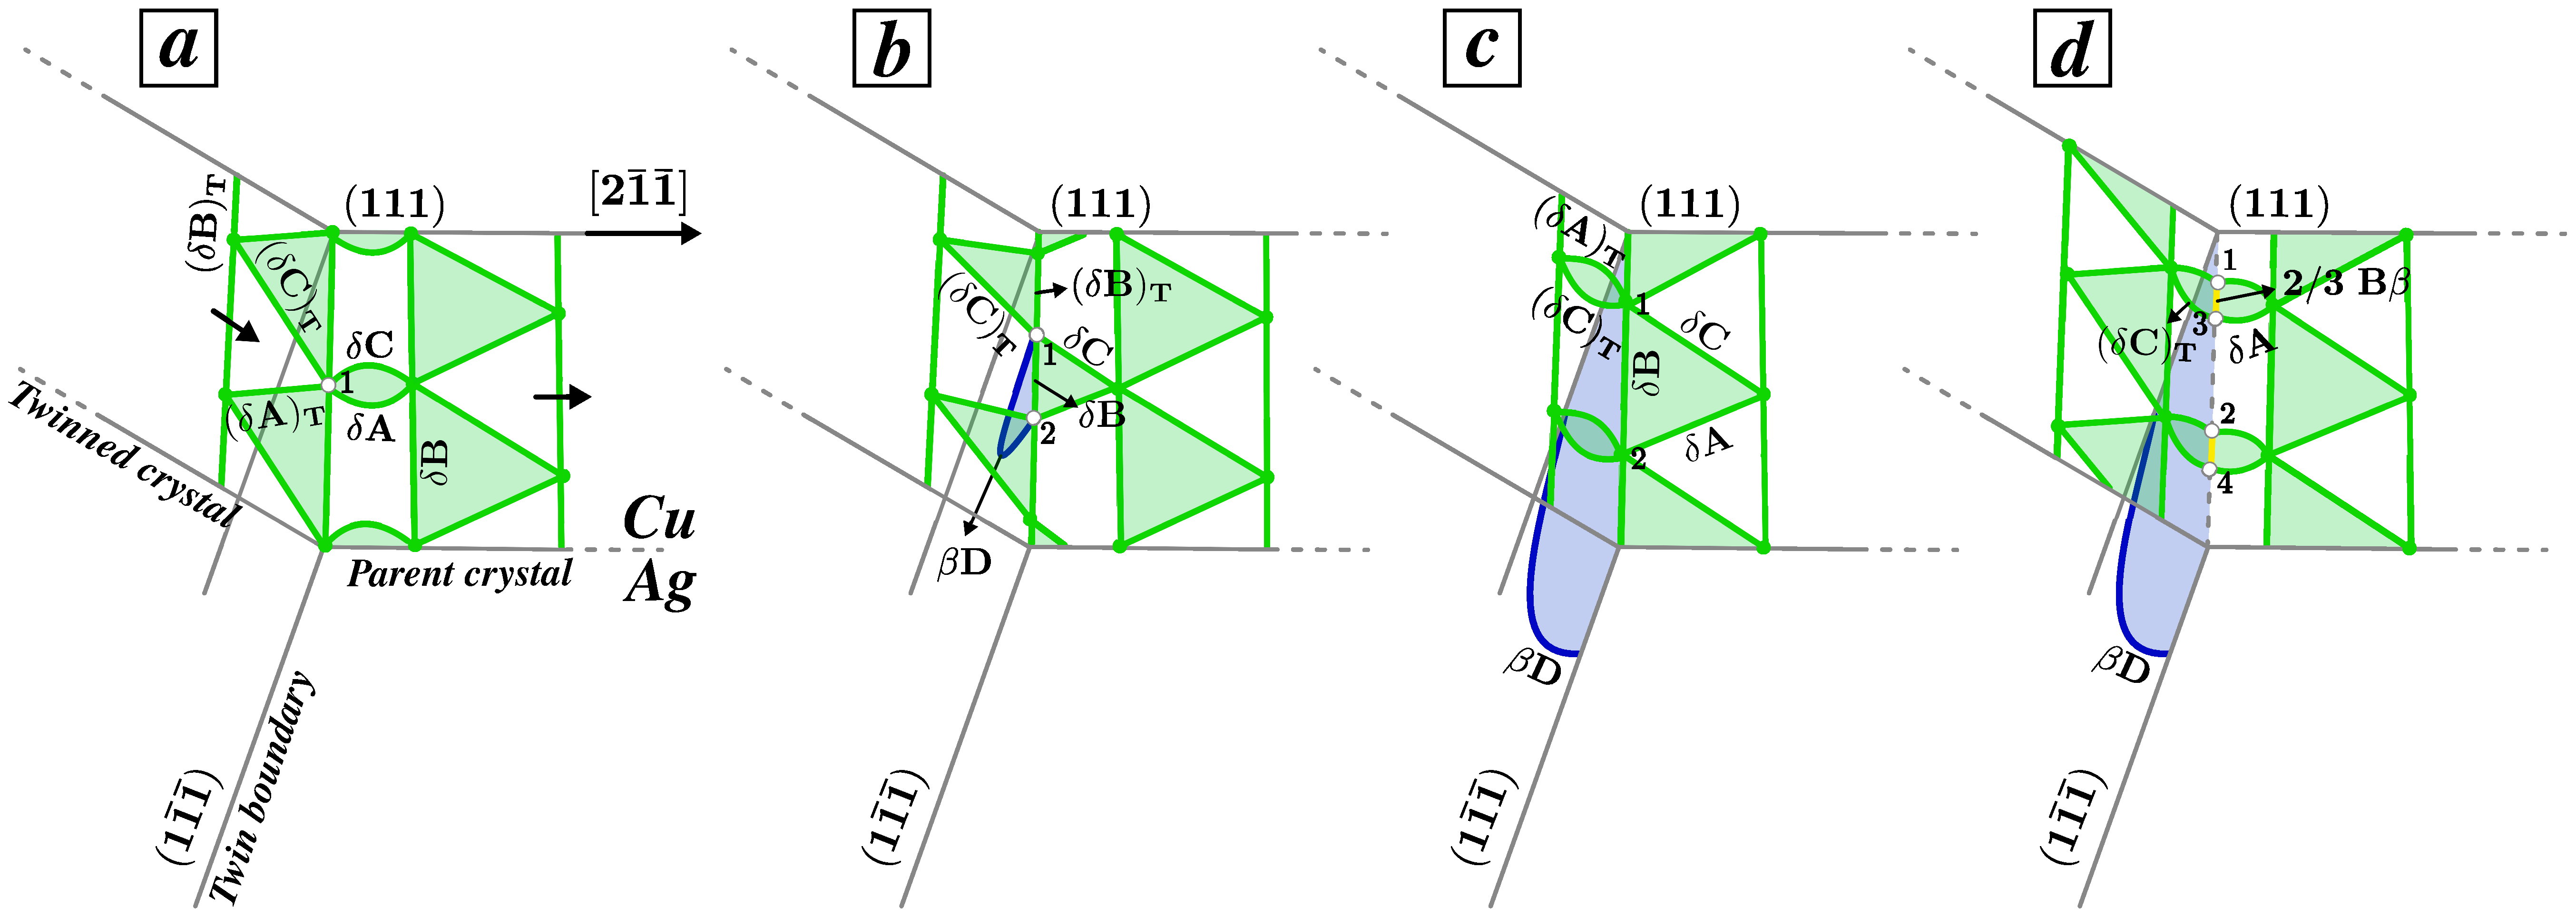
\includegraphics[width=150mm]{Pic/fig_SOR.eps} 
	\end{center}\caption{Schematic view of the mechanism leading to the transmission of the whole misfit dislocations mesh from the twinned to the perfect crystal and the nucleation of twin dislocation in the Cu layer. The line colour coding is the same as described in Fig.\ref{fig_ENT}.}\label{fig_SOR}
\end{figure*}

Therefore, two mechanisms (one at each twin boundary) leads to the extension of the newly nucleated twin. The first one, described in Fig.\ref{fig_ENT}, corresponds to the glide, from the perfect to the twinned crystal, of the whole misfit dislocation pattern through the twin boundary. For the whole description, we choose to start from the initial configuration described in Fig.\ref{fig_ENT}.a. This is actually not the real starting configuration because when the twin is formed the position of the twin boundary does not perfectly matches with the periodicity of the misfit dislocation mesh. The real configuration after the first twinning mechanism corresponds to the one in Fig.\ref{fig_ENT}.d, but due to gliding we can assert that at one time the \ref{fig_ENT}.a configuration will be reach without the emission of a twin partial dislocation. From there, the first step will consists of the gliding of the dislocations node (represented with the white circle on Fig.\ref{fig_ENT}.a) into the twinned crystal part. This step leads to the nucleation of a twin partial along the twin boundary (), a misfit dislocation in the twinned interface plane () and a residual dislocation stopped at the twin boundary (). This dissociation operates from two nodes (1 and 2 on Fig.\ref{fig_ENT}.b) which glide respectively along two perfect lattice dislocations () locked at the twin boundary. The twin partial () as well as the misfit dislocation () still continue to extend while dissociating from the nodes 1 and 2 the two perfect dislocations () at the twin boundary (see Fig.\ref{fig_ENT}.c). This dissociation leads to the nucleation of the two misfit Shockley partial dislocations (), constituting at the interface and in the twinned part, the ``triangular'' ISF pattern. Since the misfit Shockley partial dislocations () has been nucleated, the faulted ``triangular'' pattern can glide through the twin boundary (see Fig.\ref{fig_ENT}.d). Each of these misfit dislocations () can therefore can glide at the node (3 and 4) from the perfect to the twinned crystal leaving behind a residual dislocation (). Once the misfit Shockley partial dislocations () have gone through the twin boundary, the last partial dislocation () (closing the ISF in the perfect crystal) recombines locally with the residual dislocation () blocked at the twin boundary. This recombination leads from the node (3 and 4) to the formation of perfect lattice dislocations () at the twin boundary and misfit Shockley partial dislocations (), thereby closing the ``triangular'' ISF pattern in the twinned crystal part. At the end of this step, all the misfit dislocations mesh crosses the twin boundary. The two perfect lattice dislocations () has been formed and regroup in one initial node. The whole system is therefore returned into the initial configuration (see Fig.\ref{fig_ENT}.a), however during this process a twin partial has been produced, thus participating to the twin extension. 

The second mechanism operating through the second twin boundary, corresponds this time to the gliding from the twinned to the perfect crystal of the whole misfit dislocation pattern (see Fig.\ref{fig_SOR}). To describe this second mechanism, we start from the configuration in Fig.\ref{fig_SOR}.a. As it was discussed earlier, this configuration corresponds to an ideal case which the system will reach. The first step consists again in the glide of the node composed of the three misfit dislocations (), from the twinned to the perfect crystal. During this step the twin partial dislocation () is nucleated and the misfit dislocations () are transmitted through the twin boundary. The twin partial dislocation () then extends from two nodes (1 and 2 in Fig.\ref{fig_SOR}.b) gliding along the direction formed by the intersection of the twin boundary and the interface plane. This dissociation operates until the misfit dislocation () is completely transmitted through the twin boundary (see Fig.\ref{fig_SOR}.c). The final step consists in the complete crossing of () misfit dislocations (remained in the twinned crystal part) through the twin boundary. This step operates also from two nodes (3 and 4) in Fig.\ref{fig_SOR}.d and leads to the nucleation of a residual dislocation () connecting these two nodes. This residual dislocation () is locked at the interface and permits the full transmission of () misfit dislocations. Once these two last dislocations has been transmitted, the full misfit dislocations and ``triangular'' ISF pattern crossed the twin boundary. The system is therefore returned in the configuration described in Fig.\ref{fig_SOR}.a but a twin partial has been nucleated and the twin boundary has made further moves.

\section{Summary and conclusion}
\label{part_conclusion}

\textcolor{red}{Malgré ça (slower et not sufficient to completely relax the stress) il est probable que ce mécanisme soit plus important dans les systèmes réels que le mécanisme de rebond, qui est lié à la présence de surfaces proches et aussi probablement à la vitesse de déformation importante (effet cinétique, il me semble qu'il y avait une publi de Cai la-dessus). A discuter, ici, ou dans la partie 4.2, ou dans la conclusion (ma préférence pour le moment).}

\noindent\textbf{Acknowledgements}\newline
\label{part_acknowledgements}

\appendix
\noindent\textbf{Appendix A.}\newline
\label{part_appendix}

\renewcommand\thefigure{A.\arabic{figure}} 
\setcounter{figure}{0} 
\renewcommand\theequation{A.\arabic{equation}}
\setcounter{equation}{0}

For this study, a code has been developed to identify and follow over the time the number of ``twinned" atoms, in each twin or in the whole system. This algorithm involves a post processing of output atomic positions files, once the run is done. 
\\
\\
The identification of twins is based on two key quantities, calculated for each atom $i$:
\begin{itemize}
\item the local rotation associated with plasticity $\theta_{i}^{plast}$; its calculation is detailed below;
\item the CNA parameter $ f^{CNA}_{i} $, which can be obtained directly from LAMMPS.
\end{itemize}
Indeed, to belong to a twin, an atom must fulfill both conditions:
\begin{itemize}
\item the local rotation associated with plasticity $\theta_{i}^{plast}$ must be close to the theoretical value $19.47^{\circ}$ involved by twin formation;
\item the CNA parameter must be that of a perfect FCC structure, $f^{CNA}_{i} = 1$ , since an atom inside a twin is in a perfect FCC environment.
\end{itemize}

To work properly, the code needs a reference file system corresponding to the initial state. This reference system is defined by the user; it should preferably be not deformed and must not contain dislocation. The first step of the algorithm consists in searching the nearest neighbours (inside a given cut-off radius set by the user) of each atom of the reference file system, and memorizing their identification number (ID, as assigned eg by LAMMPS) into a table. This table will be useful at different stages, especially for the transformation matrix calculation and for searching twins.
 
\paragraph{Calculation of local rotation}
To calculate the local rotation for each atom $i$, we first need to determine the transformation matrix $ F^{i} $ needed to pass from the reference system to the distorted system to be treated:
\begin{equation}
x_{k}^{i}=F_{kl}^{i}.X_{l}^{i}
\end{equation}
The calculated transformation matrix ($ F^{i} $) can be decomposed into two tensors: a rotation tensor and a deformation tensor. To extract these two tensors from the transformation matrix associated to an atom $ i $, a polar decomposition is used:
\begin{equation}
F^{i}=R^{i}.U^{i}
\end{equation}
with $ R^{i} $ being the orthogonal rotation tensor and $ U^{i} $ the symmetric right stretch tensor. \\ 
The rotation matrix can then be written as a function of the rotation angle $ \theta_{i} $ about the rotation axis, defined by the unit vector $ \overrightarrow{u} (u_{x},u_{y},u_{z})$:

\begin{equation}
	R^{i}=\begin{footnotesize}\left(
	\begin{array}{ccc}
	u_{x}^{2}(1-c)+c & u_{x}u_{y}(1-c)-u_{z}s & u_{x}u_{z}(1-c)+u_{y}s \\
	u_{x}u_{y}(1-c)+u_{z}s & u_{y}^{2}(1-c)+c & u_{y}u_{z}(1-c)-u_{x}s \\
	u_{x}u_{z}(1-c)-u_{y}s & u_{y}u_{z}(1-c)+u_{x}s & u_{z}^{2}(1-c)+c \\
	\end{array}
	\right)\end{footnotesize}
\end{equation}

with $ s=\sin(\theta_{i}) $ and $ c=\cos(\theta_{i}) $. \\
The local rotation $ \theta_{i} $ associated to an atom $ i $ is next calculated from the trace of $ R^{i} $:
\begin{equation}
	\cos(\theta_{i})=\frac{1}{2}\left[tr\left(R^{i}\right)-1\right]
\end{equation}
To determine the sign of $ \theta_{i} $, the orientation of the rotation axis $ \overrightarrow{u}(u_{x},u_{y},u_{z}) $ and $\sin(\theta_{i}) $ are also extracted from the rotation matrix $ R^{i} $.
\\
However, this calculated rotation extracted from the rotation matrix comprises not only the local rotation due to plasticity ($ \theta_{i}^{plast} $) but also a global rotation ($ \theta_{o} $) of the whole system which is induced in our case by the presence of periodic boundary conditions. The local rotation $ \theta_{i} $ can therefore be expressed as follows:
\begin{equation}\label{thetatot}
\theta_{i}=\theta_{o}+\theta_{i}^{plast}
\end{equation}
$ \theta_{o} $ can be calculated by averaging $ \theta_{i} $ over all atoms that have not been plastically deformed, for which $ \theta_{i}^{plast}=0 $. These atoms are identified through a regular monitoring of the CNA parameter: it should remain zero for atoms that have not been plastically deformed. Once $ \theta_{o} $ is determined, $ \theta_{i}^{plast} $ is obtained from equation (\ref{thetatot}).


\paragraph{Twin search algorithm}
When the local plastic rotation is known, the twin search can begin. We first create a function $ f^{twin} $ which will return, for an atom $ i $, the twin ID to which it belongs. If the atom does not belong to a twin, the result will be zero ($ f^{twin}_{i}=0$). For twin search, the atoms of the system are first scanned randomly until one is found respecting both conditions described above ($ \theta_{i}^{plast} \approx 19.47^{\circ} $ and $f^{CNA}_{i}=1 $). The atom $i$ is then considered as belonging to a new twin, to which an ID is assigned, and $f^{twin}_{i}$ is set to this ID. The next operation consists in searching all the other atoms in that same twin. To do this, starting from the atom $ i $ we look step by step if neighbour atoms are in the twin configuration (see Fig. \ref{fig_A1}). If some neighbour atoms fulfil the twin conditions, they are assigned the corresponding twin ID and they are memorized to be later analysed. This operation is repeated until all the atoms belonging to the twin are identified. We can therefore randomly search for another atom corresponding to a twin type configuration and make a new step by step search. When all the atoms of the system have been analysed, all twins have been found and the ID of the last identified twin corresponds to the number of twins in the whole system.

\begin{figure}[!h]
	\begin{center}
		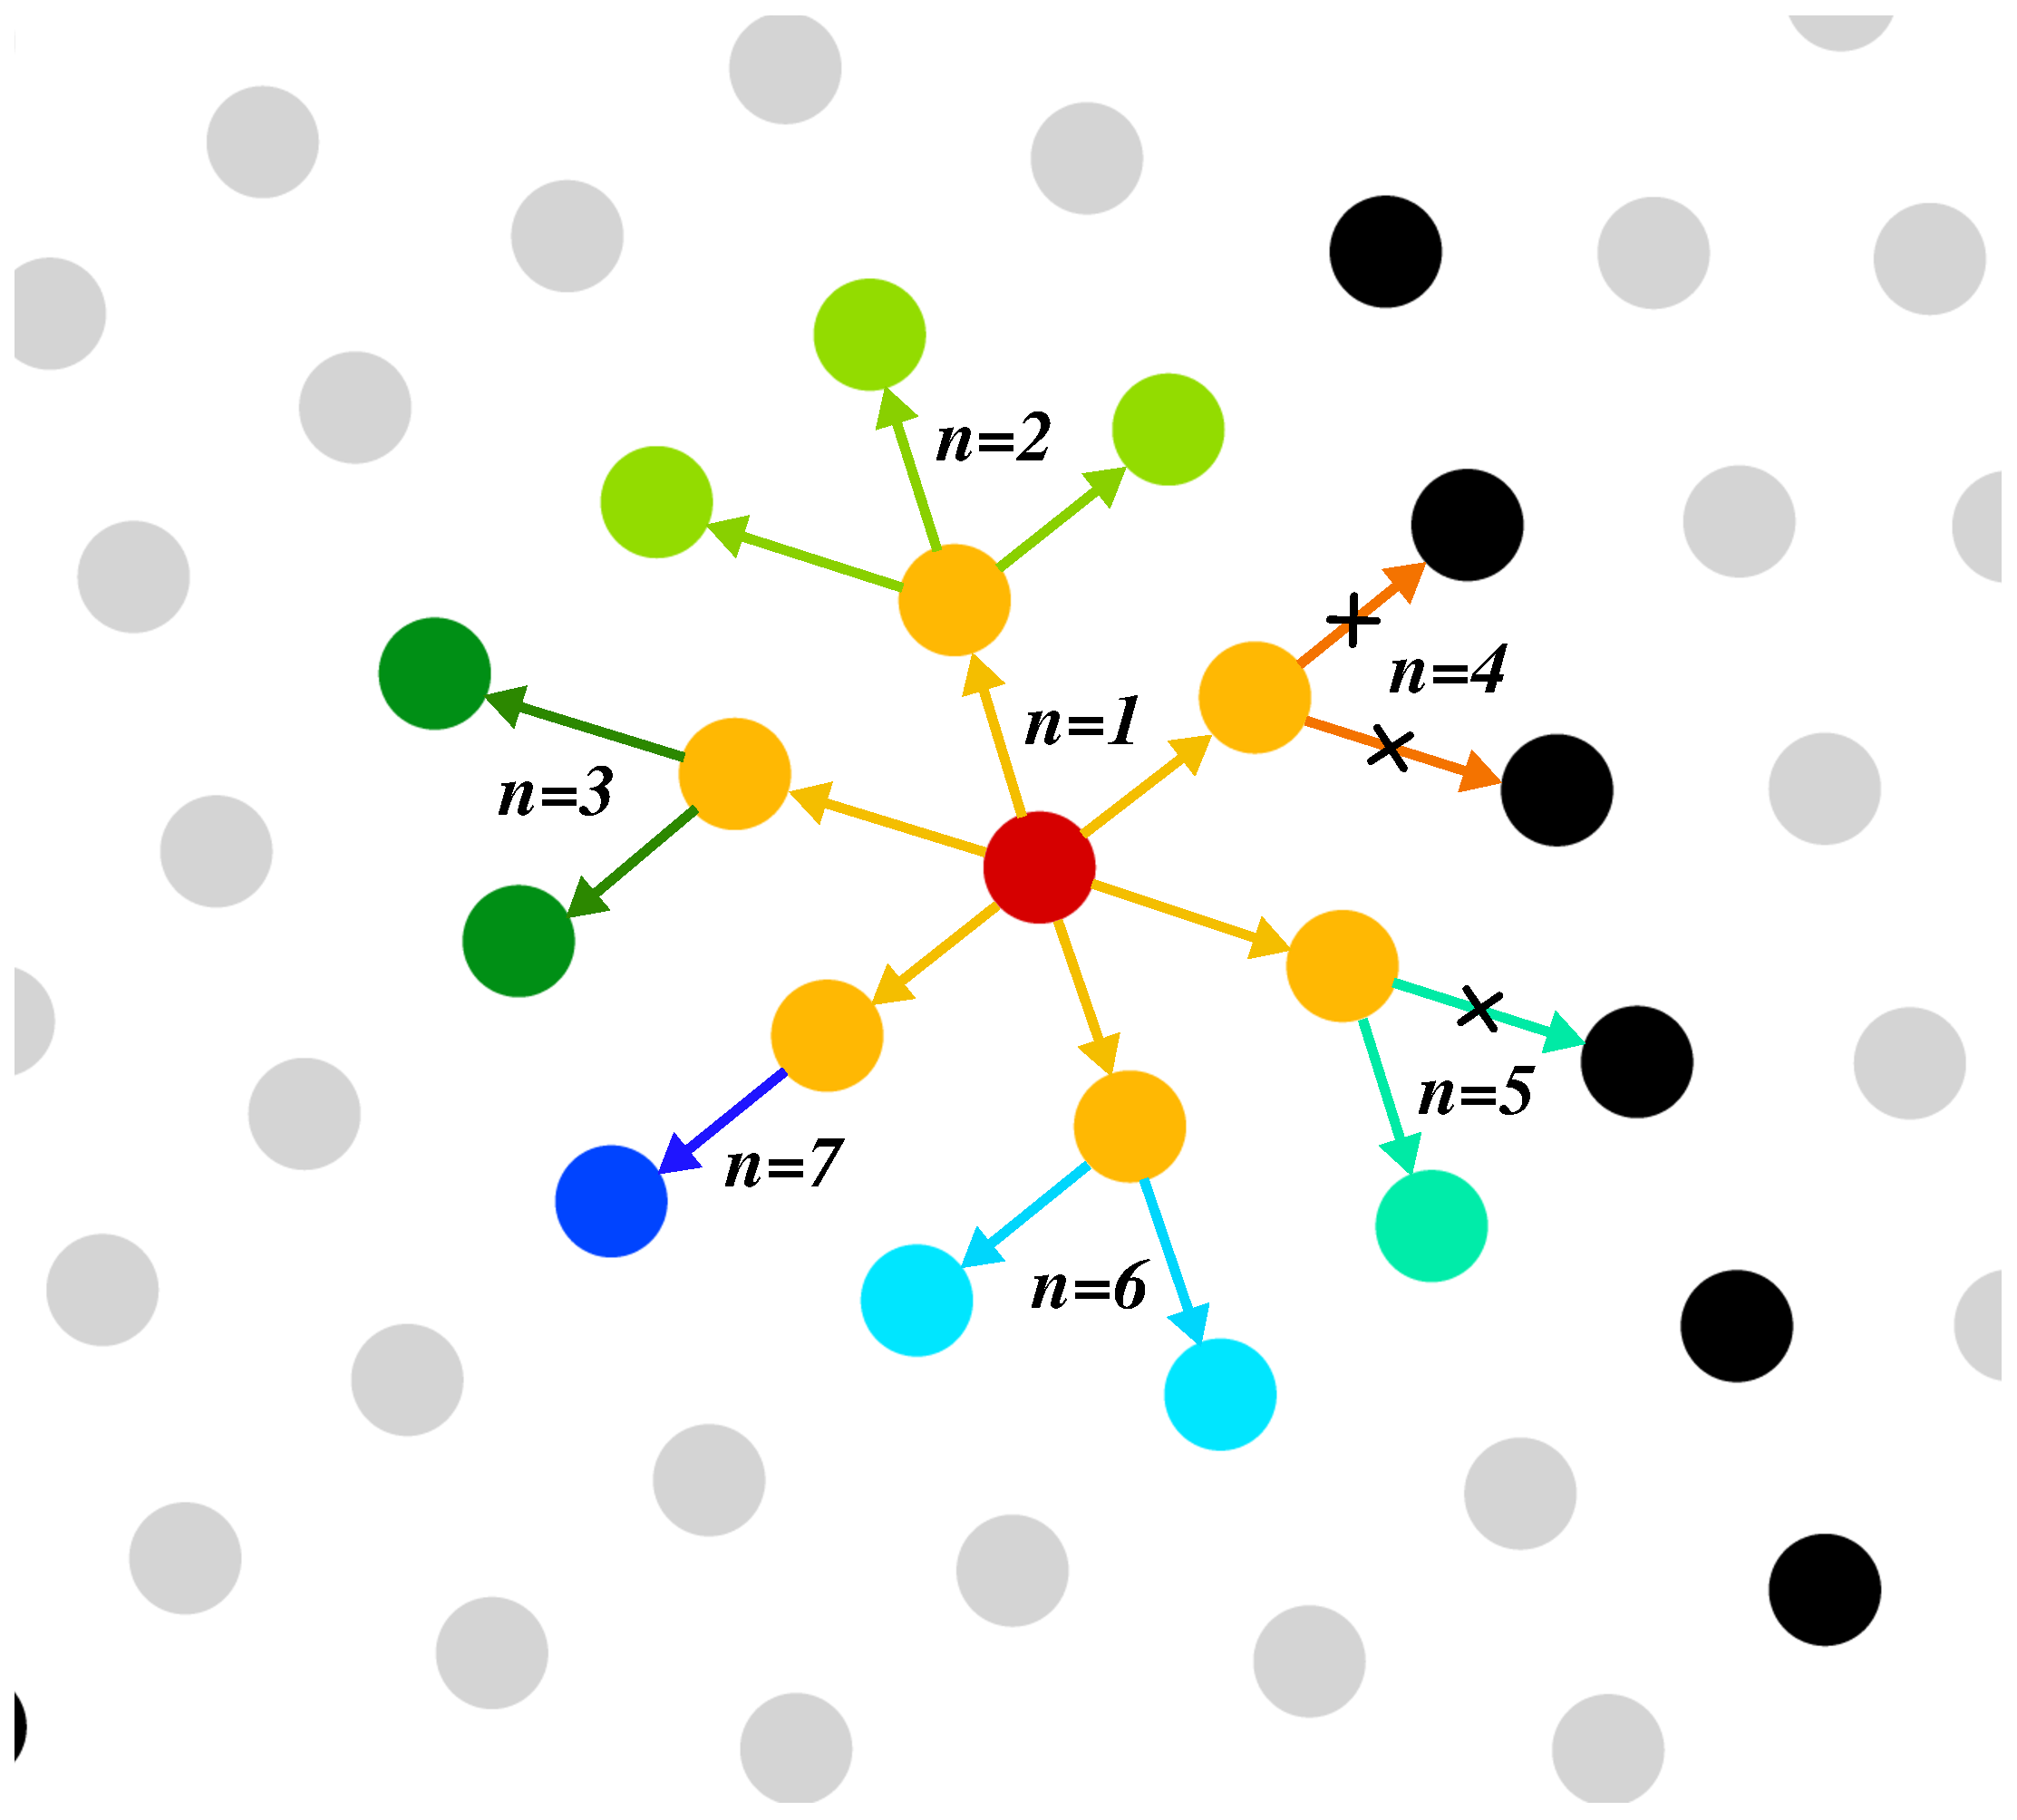
\includegraphics[width=60mm]{Pic/fig_A1.eps} 
	\end{center}
	\caption{Seven first iterations of the step by step twin identification algorithm; in light gray the atoms corresponding to a perfect FCC crystal structure (CNA = 1) and in black the atoms belonging to a stacking fault (CNA = 2). Colours are superimposed to display the growth of the detected twinned zone.}\label{fig_A1}
\end{figure}

\paragraph{Identification of twin boundaries}
Atoms in a CTB are characterized by a CNA parameter equal to 2, corresponding to a compact hexagonal local structure. Thus they have not been identified in the previous step of the algorithm. Here again, a function ($ f^{tb} $) is created, which will return, for an atom $ i $ belonging to a twin boundary, the ID of the twin considered. For example, if an atom $ i $ is in the boundary of the twin whose ID is 2 then $ f^{tb}_{i}=2 $. On the other hand, if the atom is not in a twin boundary, the returned value will be zero ($ f^{tb}_{i}=0 $). Here only atoms whose CNA parameter is equal to 2 are scanned. These atoms can belong either to a stacking fault (ISF), generated by one Shockley dislocation, or to a twin boundary. To differentiate between ISF and CTB, it is sufficient to look if a twin has been identified in the close proximity of the scanned atom; if it is the case, the ID of the nearby twin will be assigned to it ($ f^{tb}_{i}=ID $). Thus, an atom whose CNA parameter is 2 is considered in a twin boundary if it has at least two neighbour atoms $ j $ belonging to a twin ($ f^{twin}_{j}=ID $) and two others belonging to a non-twinned crystal ($ f^{twin}_{j}=0 $). 

\paragraph{Final check}
In some cases, a group of atoms may be erroneously identified as a twin by the algorithm. It is the case for example for atoms crossed by a full lattice dislocation: the local rotation induced by this dislocation is close to $ 19.47^{\circ} $ and after the passage of the dislocation these atoms have again the perfect CFC structure. Therefore, this group of atoms has been identify as a twin by the algorithm but can not be considered as a ``real" twin and must be removed from the list. Such a group of atoms has no twin boundary associated to it, so that the final check is to test if the twins identified by the algorithm have a twin boundary associated with them, in which only case they are kept in the twin list.
\newline

\noindent\textbf{References}
\bibliographystyle{elsarticle-num}
\bibliography{Bib/test_bib}


\end{document}
\endinput


